\chapter{Online Deployment}%
\label{sec:operation}



This \textcolor{red}{section reports the \rnn{}} operation in both 2017
(Section~\ref{ssec:2017_ringer_operation}) and 2018
(Section~\ref{ssec:2018_ringer_operation}) data acquisition periods. The operation efficiencies
\textcolor{red}{are computed with respect to offline electrons, as} indicated in
Section~\ref{ssec:dataset}\footnote{For efficiency measurements in this section,
	fake electrons are selected always employing \veto\vloose{} offline likelihood
	working point.}. Firstly, we detail the algorithm cycle during Run~2
(Section~\ref{ssec:run2_rnn_cycle}).

\section{Run~2 \rnn{} Cycle}\label{ssec:run2_rnn_cycle}

\textcolor{red}{During the Run 2, the actual} \rnn{} \textcolor{red}{implementation} 
%The \rnn cycle 
can be partitioned into four chronological stages:

\begin{enumerate}[i]
  \item A development stage up to early 2017, where the \rnn{}
      potential was estimated from trigger emulation and data reprocessing;
  \item The commissioning stage (\SI{5.4}{\per\femto\barn}) occurred in
      early 2017 runs, where all primary
      triggers were duplicated with either the \rnn{} or cut-based algorithms
      operating in the \fastcalo{};
  \item The operation of the method as the baseline trigger, which occurred after 2017 Technical Stop 1 (TS1). For
    monitoring purposes, and to allow precise statistical evaluation of eventual
    disagreements between the \fastcalo{} \textcolor{red}{methods from an} offline
    perspective (Section~\ref{sec:off_ana}), a duplicated trigger pair, i.e.
    with and without \rnn{}, was kept operating unprescaled during this period
    (\SI{39.0}{\per\femto\barn}). Here, we compare the efficiencies of the
    duplicated triggers in 2017 (Section~\ref{ssec:2017_ringer_operation});
  \item Finally, the duplicated trigger was removed for 2018 operation.
    Therefore, we evaluate 2018 \rnn{} operation relying on a comparison with
    2017 efficiency in Section~\ref{ssec:2018_ringer_operation}.
\end{enumerate}

\section{2017 Operation}\label{ssec:2017_ringer_operation}

% FIXME Don't forget that there are some of these plots that were already
% approved.

%A backup trigger ($\text{e28\_lhtight\_nod0\_ivarloose}$) was employed for
A backup trigger (offline tight) was employed for
monitoring purposes after the TS1. During the monitoring process, a similar
operation of both triggers was observed in terms of signal efficiency using the
integrated luminosity along the period, as shown in
Figure~\ref{fig:e28_triggers}. The trigger
turn-on curves exhibit similar profile. In $\eta$, \rnn{} shows a reasonably symmetric
profile with respect to positive and negative $\eta$, while a
\SI{3}{\%} efficiency loss is observed at $-2.01<\eta<-1.81$\footnote{The cause for this efficiency loss is unknown, but we expect it to be caused by a change in either one or more of the ratio profiles reconstructed by the FastCalo.}. In addition, a difference of about
half to one percentage point may be observed in $\eta$ regions \textcolor{red}{(crack regions)} with deterioration in the calorimeter
response ($1.37 < \abseta < 1.52$ and $2.37 < \abseta < 2.45$). Besides
aforementioned points, overall efficiency fluctuations are smaller than a few
per-mill. Although a slight more prominent efficiency loss with respect to
\avgmu{} is observed in Figure~\ref{fig:e28_comp_mu} for the \rnn{} trigger, the
electron efficiency was kept nearly the same. Such loss occurs after the
linear threshold correction limit that was employed during 2017 ($\avgmu=40$).

Other important triggers were assessed by comparing the trigger efficiencies on
2017 data collected before and after switching to the \rnn{} algorithms.  As it can be
observed in Figure~\ref{fig:2017_ts1}, the electron efficiency was also kept
nearly unchanged for relevant single electron triggers. Note that results in
this plot are computed with two different data taking periods (with or
without the \rnn{} algorithm). The e17\_lhvloose\_nod0 trigger shows the
\textcolor{red}{efficiency in the lowest-energy-threshold} 
% efficiency of the legs in the lowest-energy-threshold 
unprescaled two electron trigger.
Similar behavior was observed during data collection for all monitored triggers.


\begin{figure}[h!tb]
  \begin{center}
  \begin{subfigure}[c]{.48\textwidth}
  \centering
  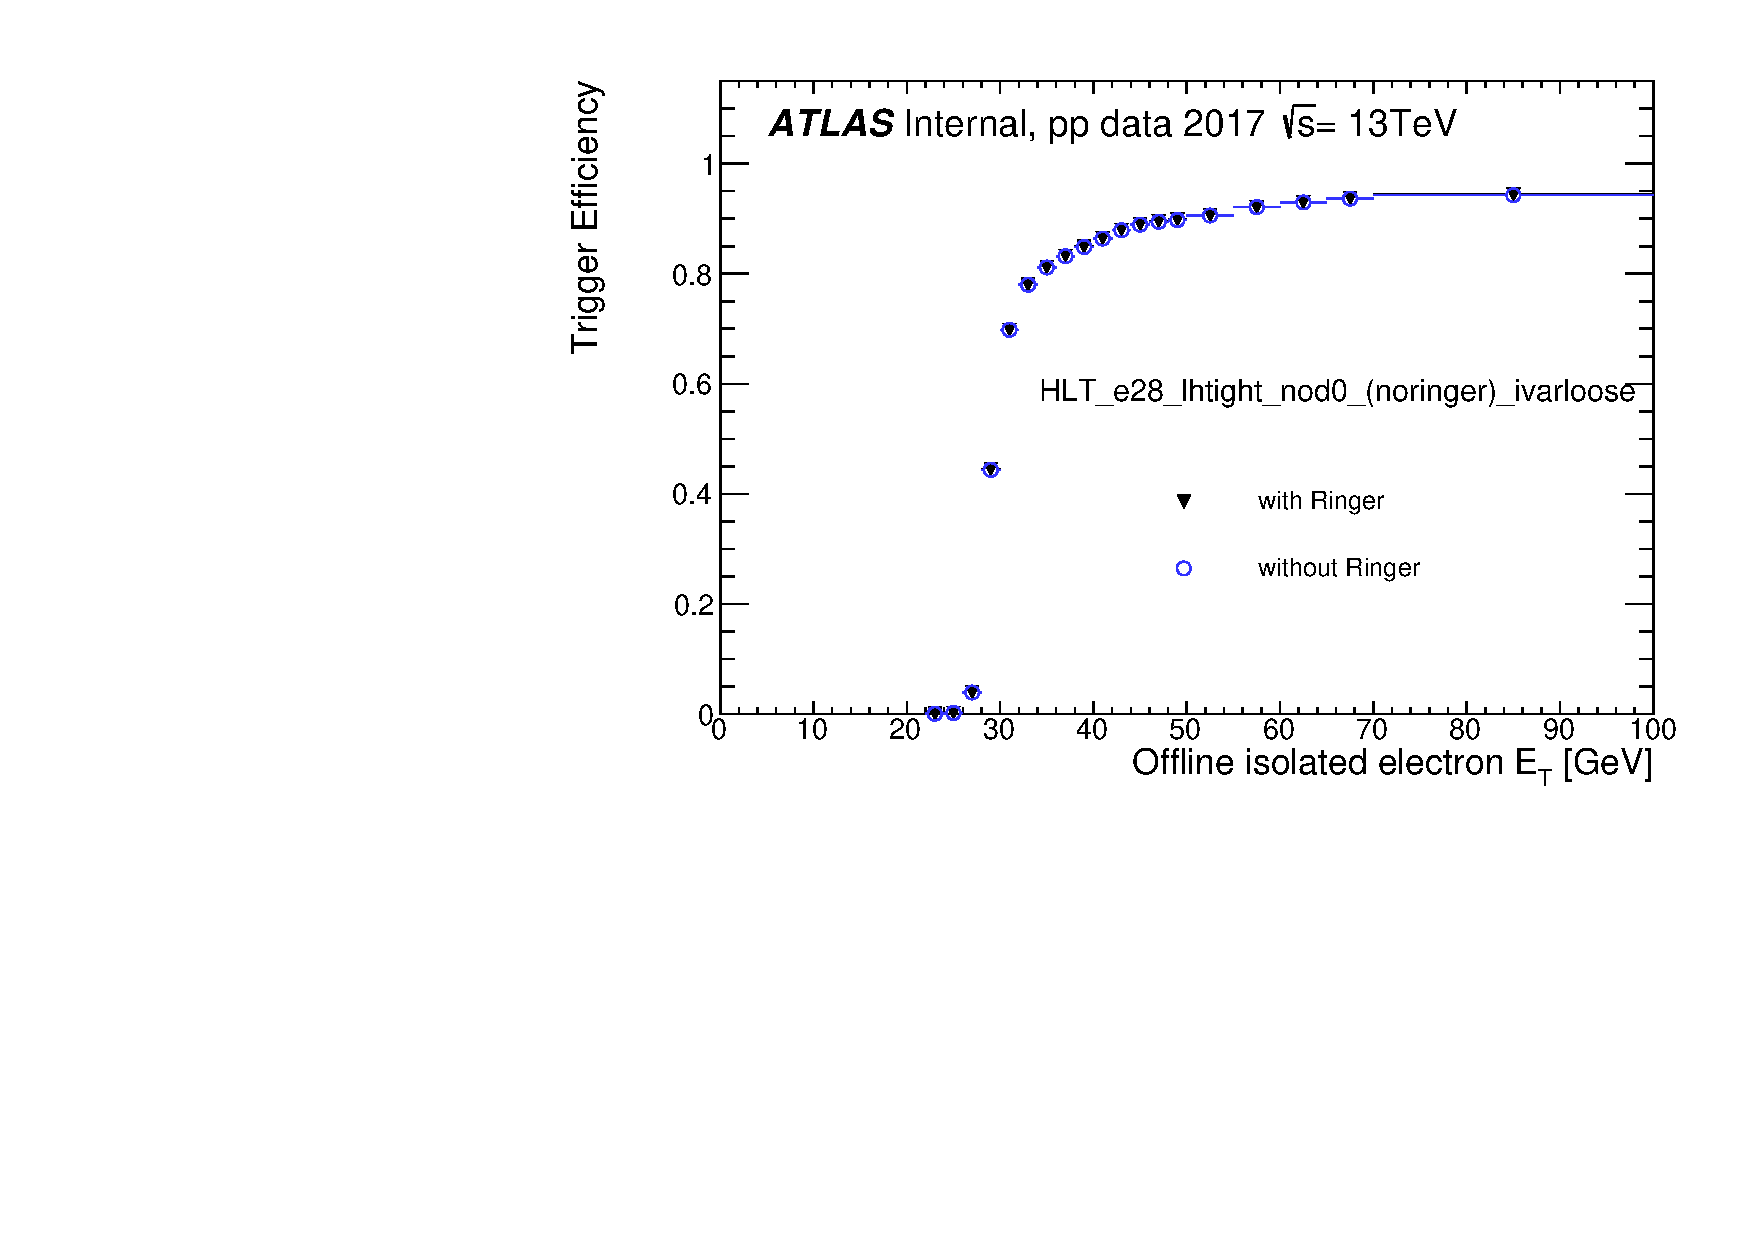
\includegraphics[width=\textwidth]{sections/operation/figures/efficiencies/eff_EGAM1_e28_ringer_and_noringer_2017_after_ts1_HLT_et.pdf}
  \caption{}%

  \end{subfigure}
  \hfill
  %\hspace{0.01\textwidth}
  \begin{subfigure}[c]{.48\textwidth}
  \centering
  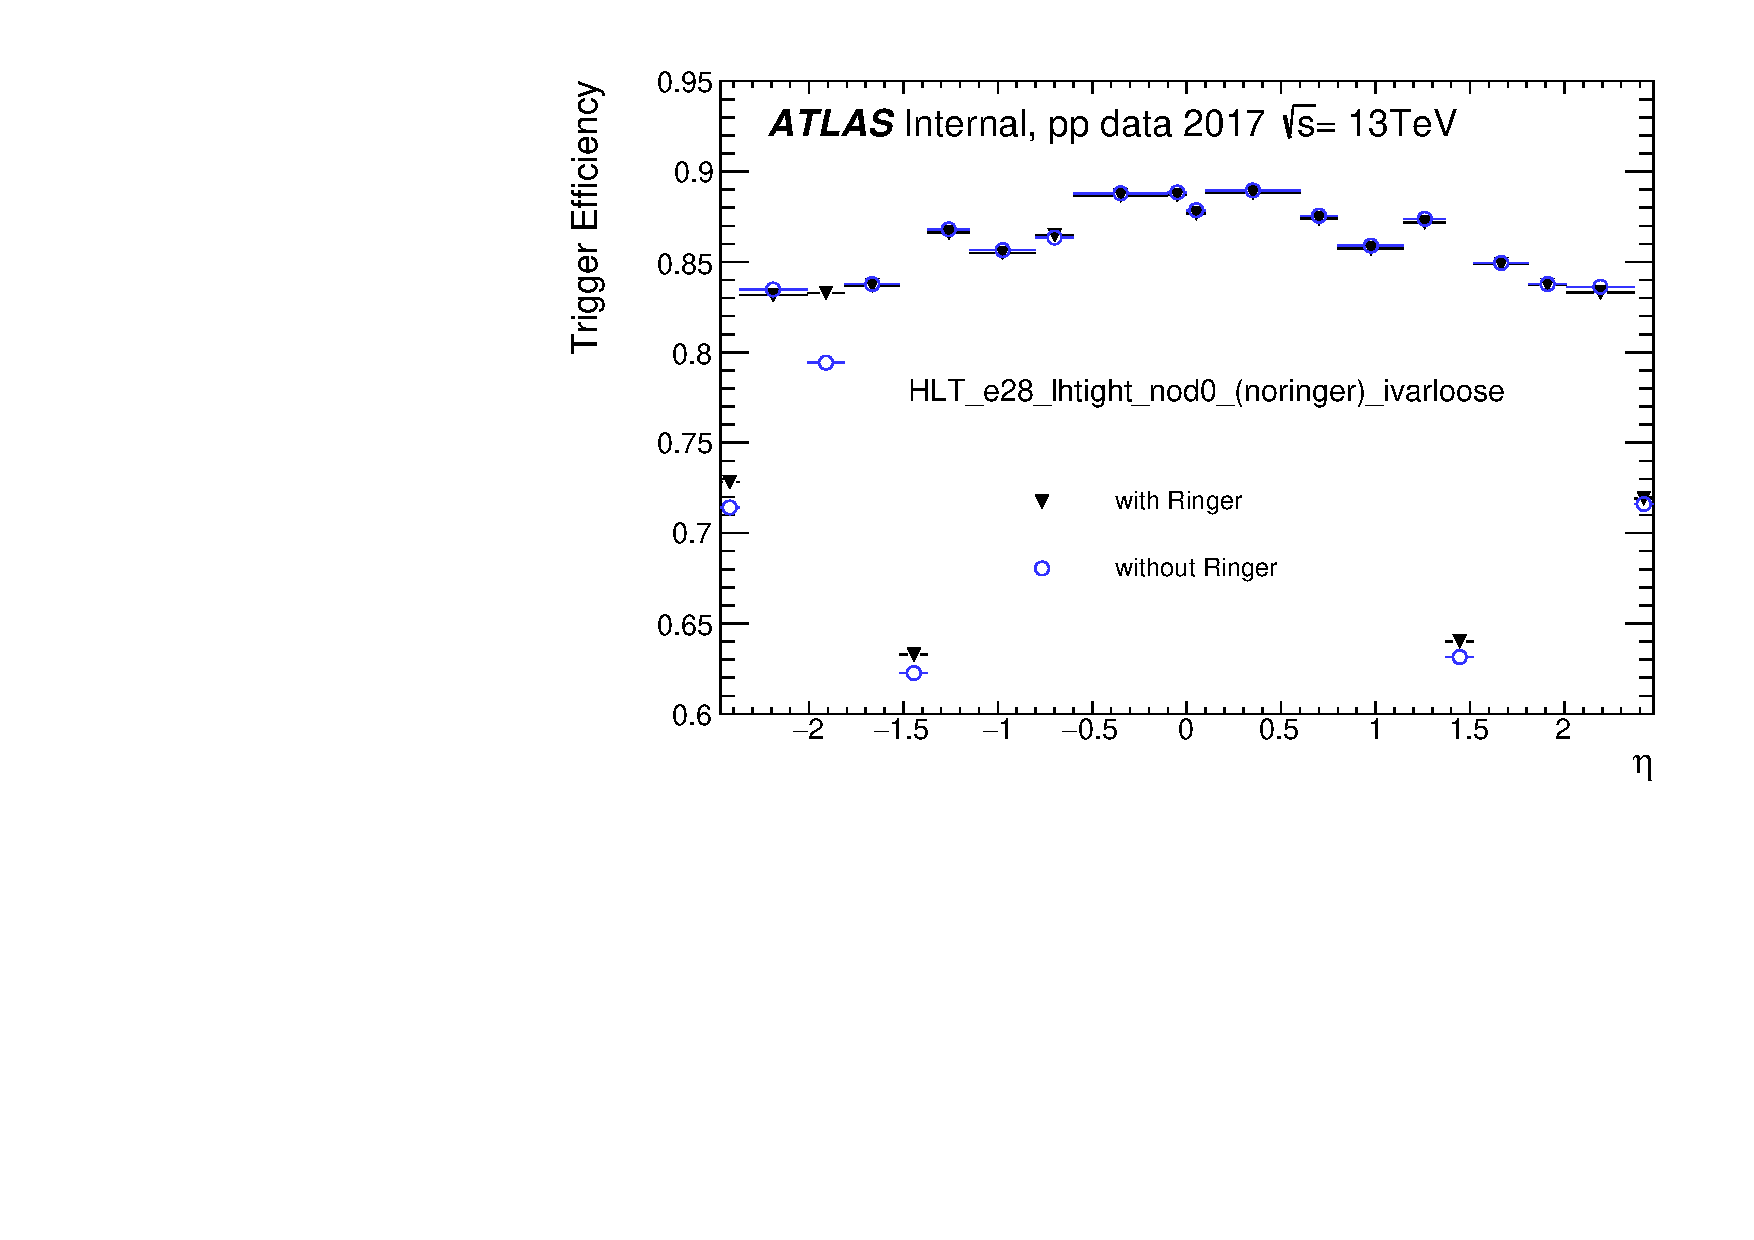
\includegraphics[width=\textwidth]{sections/operation/figures/efficiencies/eff_EGAM1_e28_ringer_and_noringer_2017_after_ts1_HLT_eta.pdf}
  \caption{}%
  %\label{fig:e28_comp_eta}
  \end{subfigure} \\
  \begin{subfigure}[c]{.48\textwidth}
  \centering
  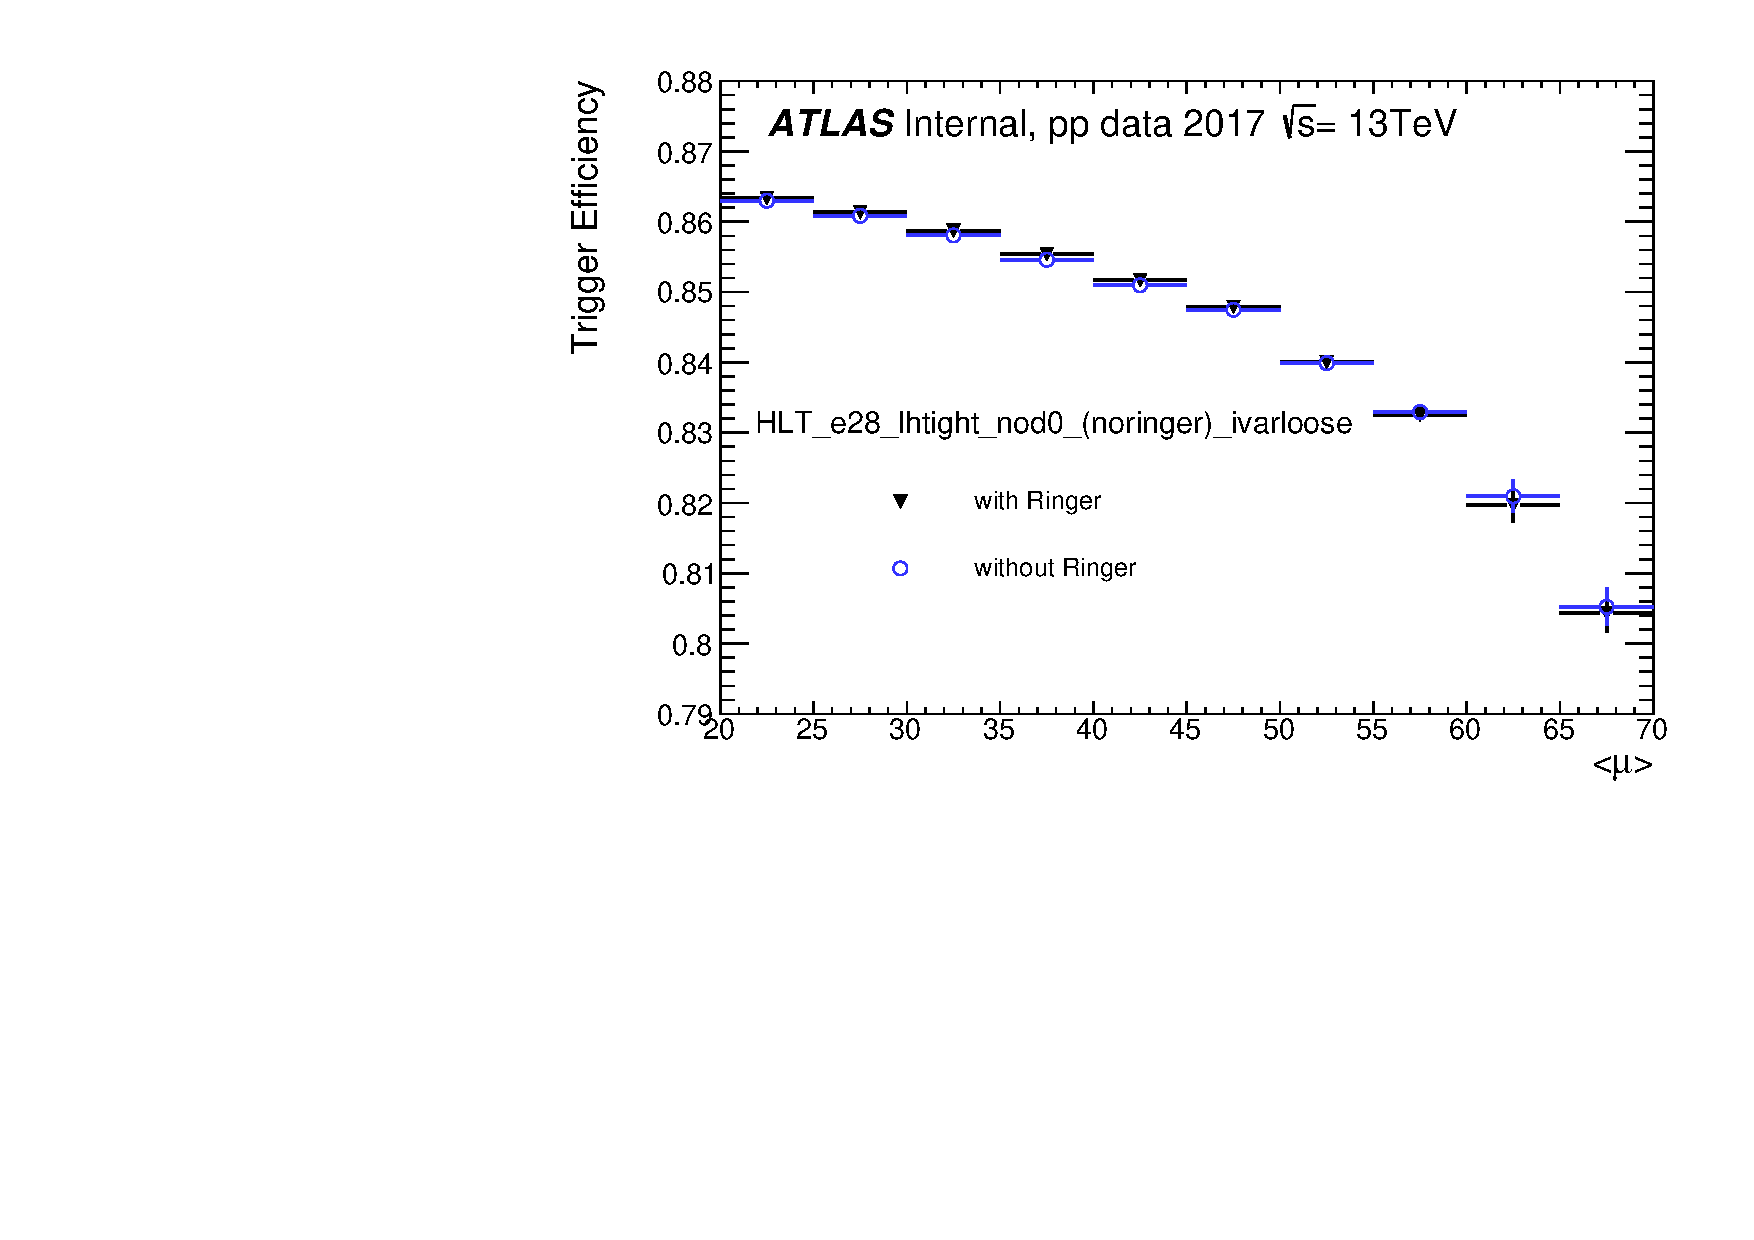
\includegraphics[width=\textwidth]{sections/operation/figures/efficiencies/eff_EGAM1_e28_ringer_and_noringer_2017_after_ts1_HLT_mu.pdf}
  \caption{}%
  \label{fig:e28_comp_mu}
  \end{subfigure}
  \caption{\label{fig:e28_triggers}HLT electron efficiency as a function of \et{}
    (a), \eta{} (b) and \avgmu{} (c) for the duplicated single electron trigger
    requiring $\et{} > \SI{28}{\GeV}$ and \tight{} selection with and without the
    \rnn{} algorithm. Efficiencies are measured employing 2017 data collected
    after TS1.}
  \end{center}
\end{figure}
  
\begin{figure}[h!tb]
  \begin{center}
  \begin{subfigure}[c]{.48\textwidth}
  \centering
  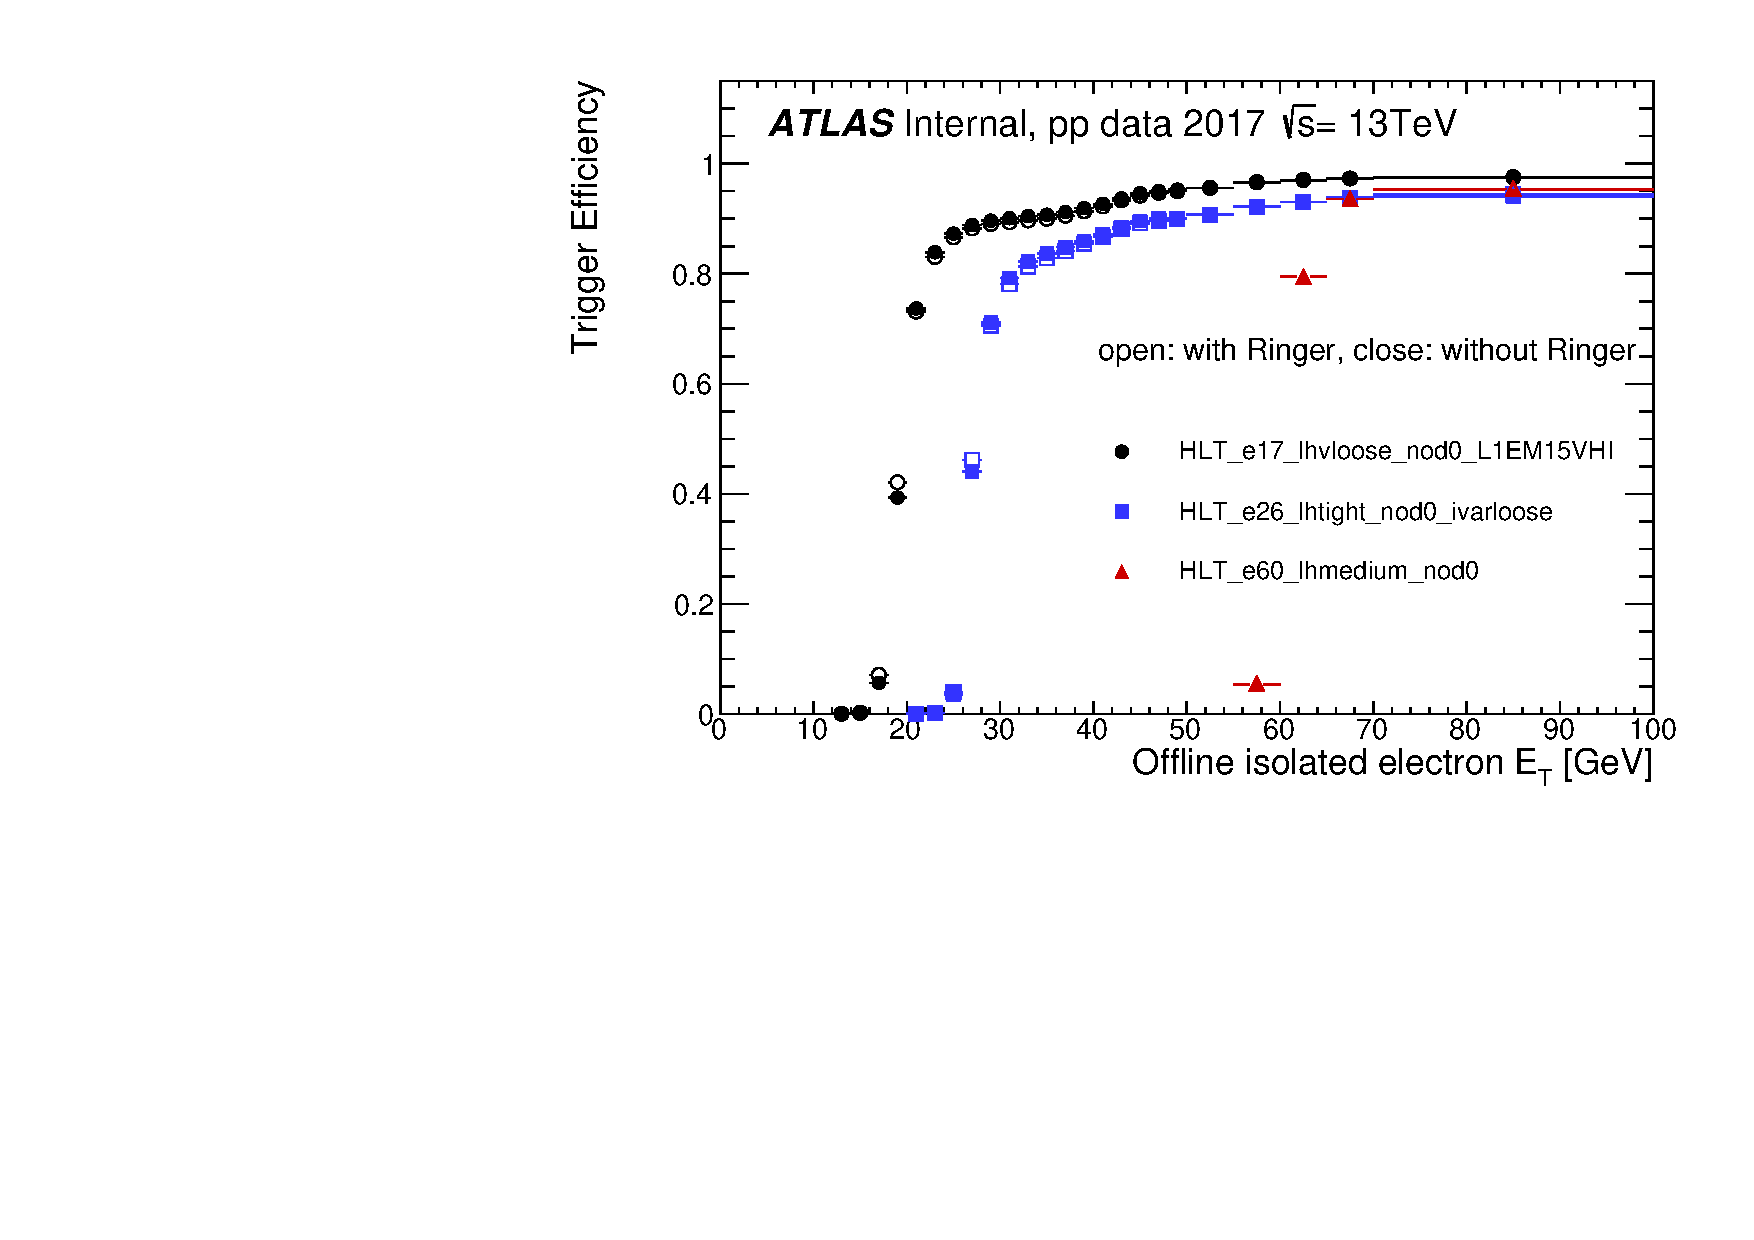
\includegraphics[width=\textwidth]{sections/operation/figures/efficiencies/eff_EGAM1_e17_e26_e60_2017_before_and_after_ts1_et.pdf}
  \caption{}%
  \end{subfigure}
  \hfill
  %\hspace{0.01\textwidth}
  \begin{subfigure}[c]{.48\textwidth}
  \centering
  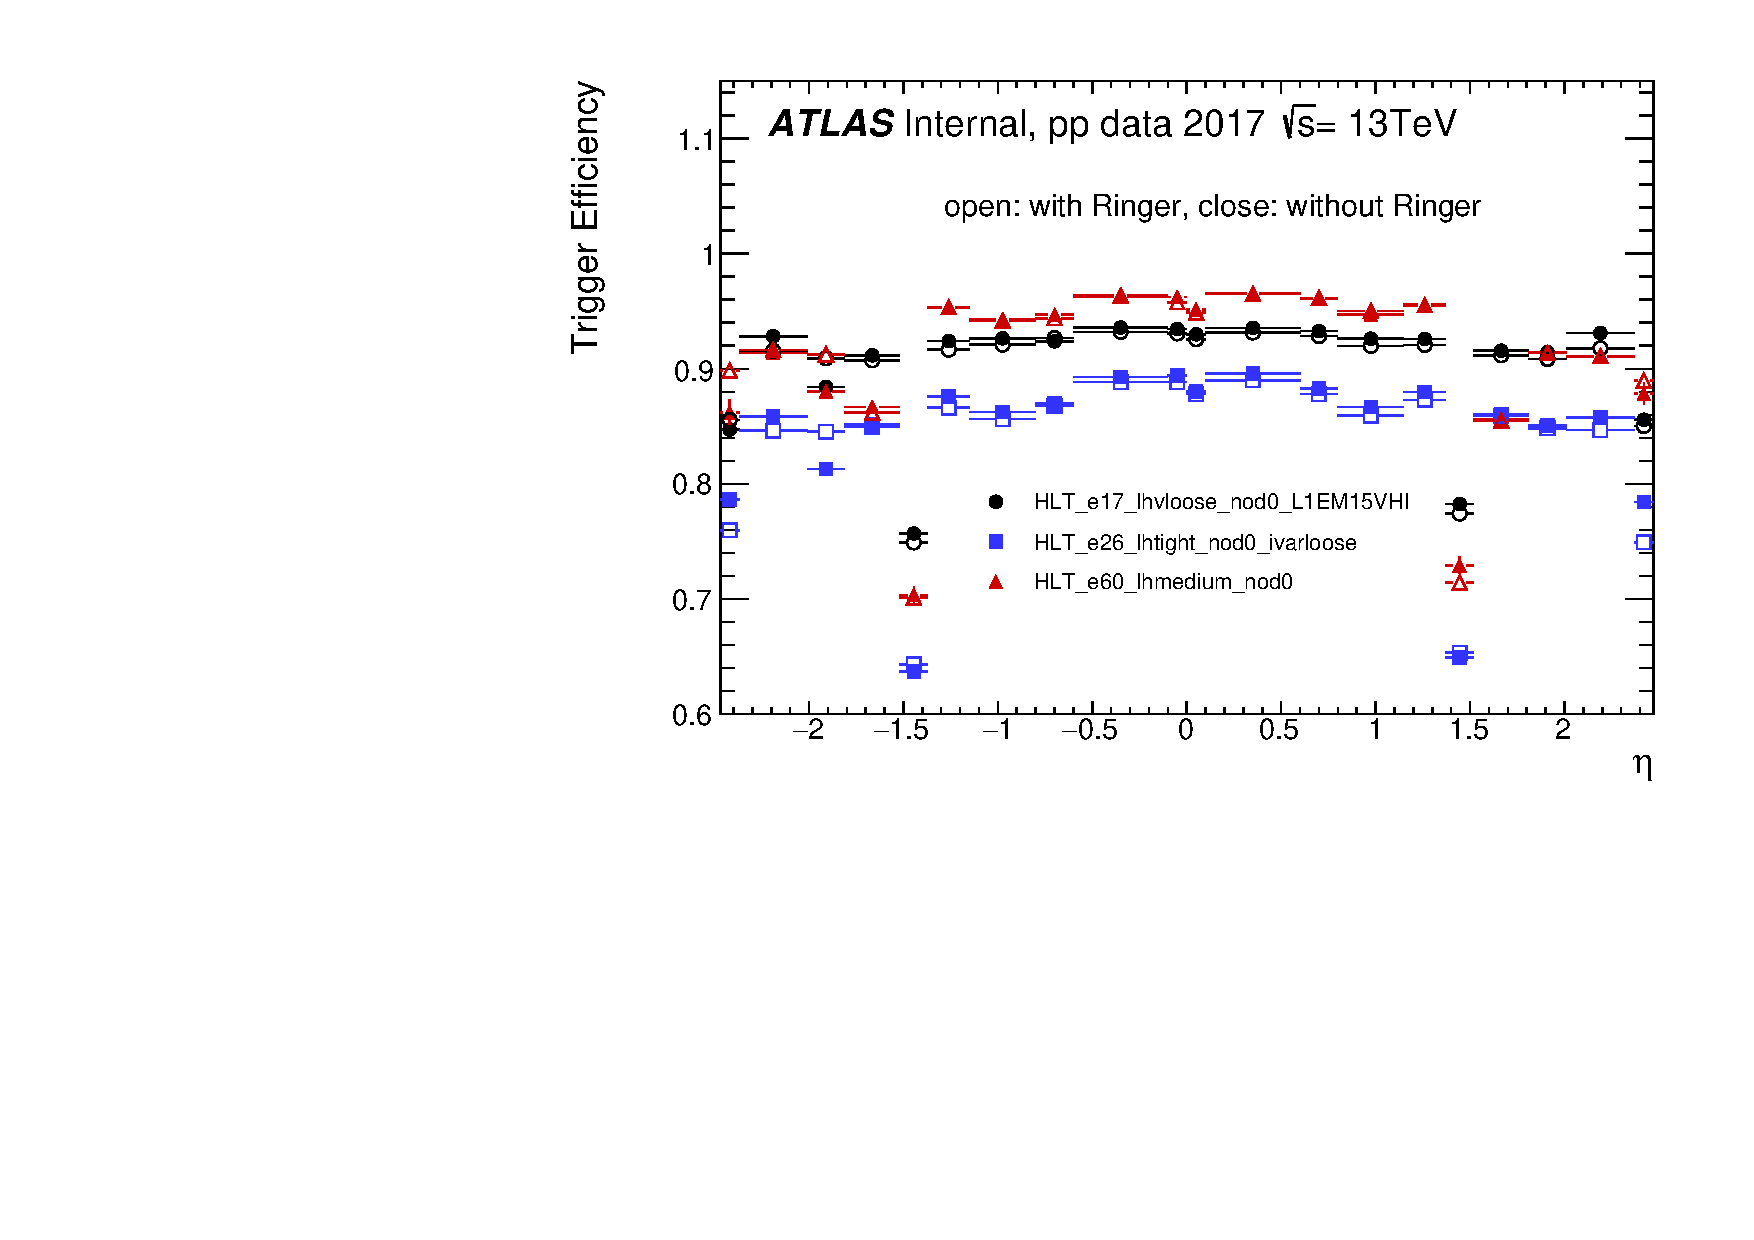
\includegraphics[width=\textwidth]{sections/operation/figures/efficiencies/eff_EGAM1_e17_e26_e60_2017_before_and_after_ts1_eta.pdf}
  \caption{}%
  \end{subfigure} \\
  \begin{subfigure}[c]{.48\textwidth}
  \centering
  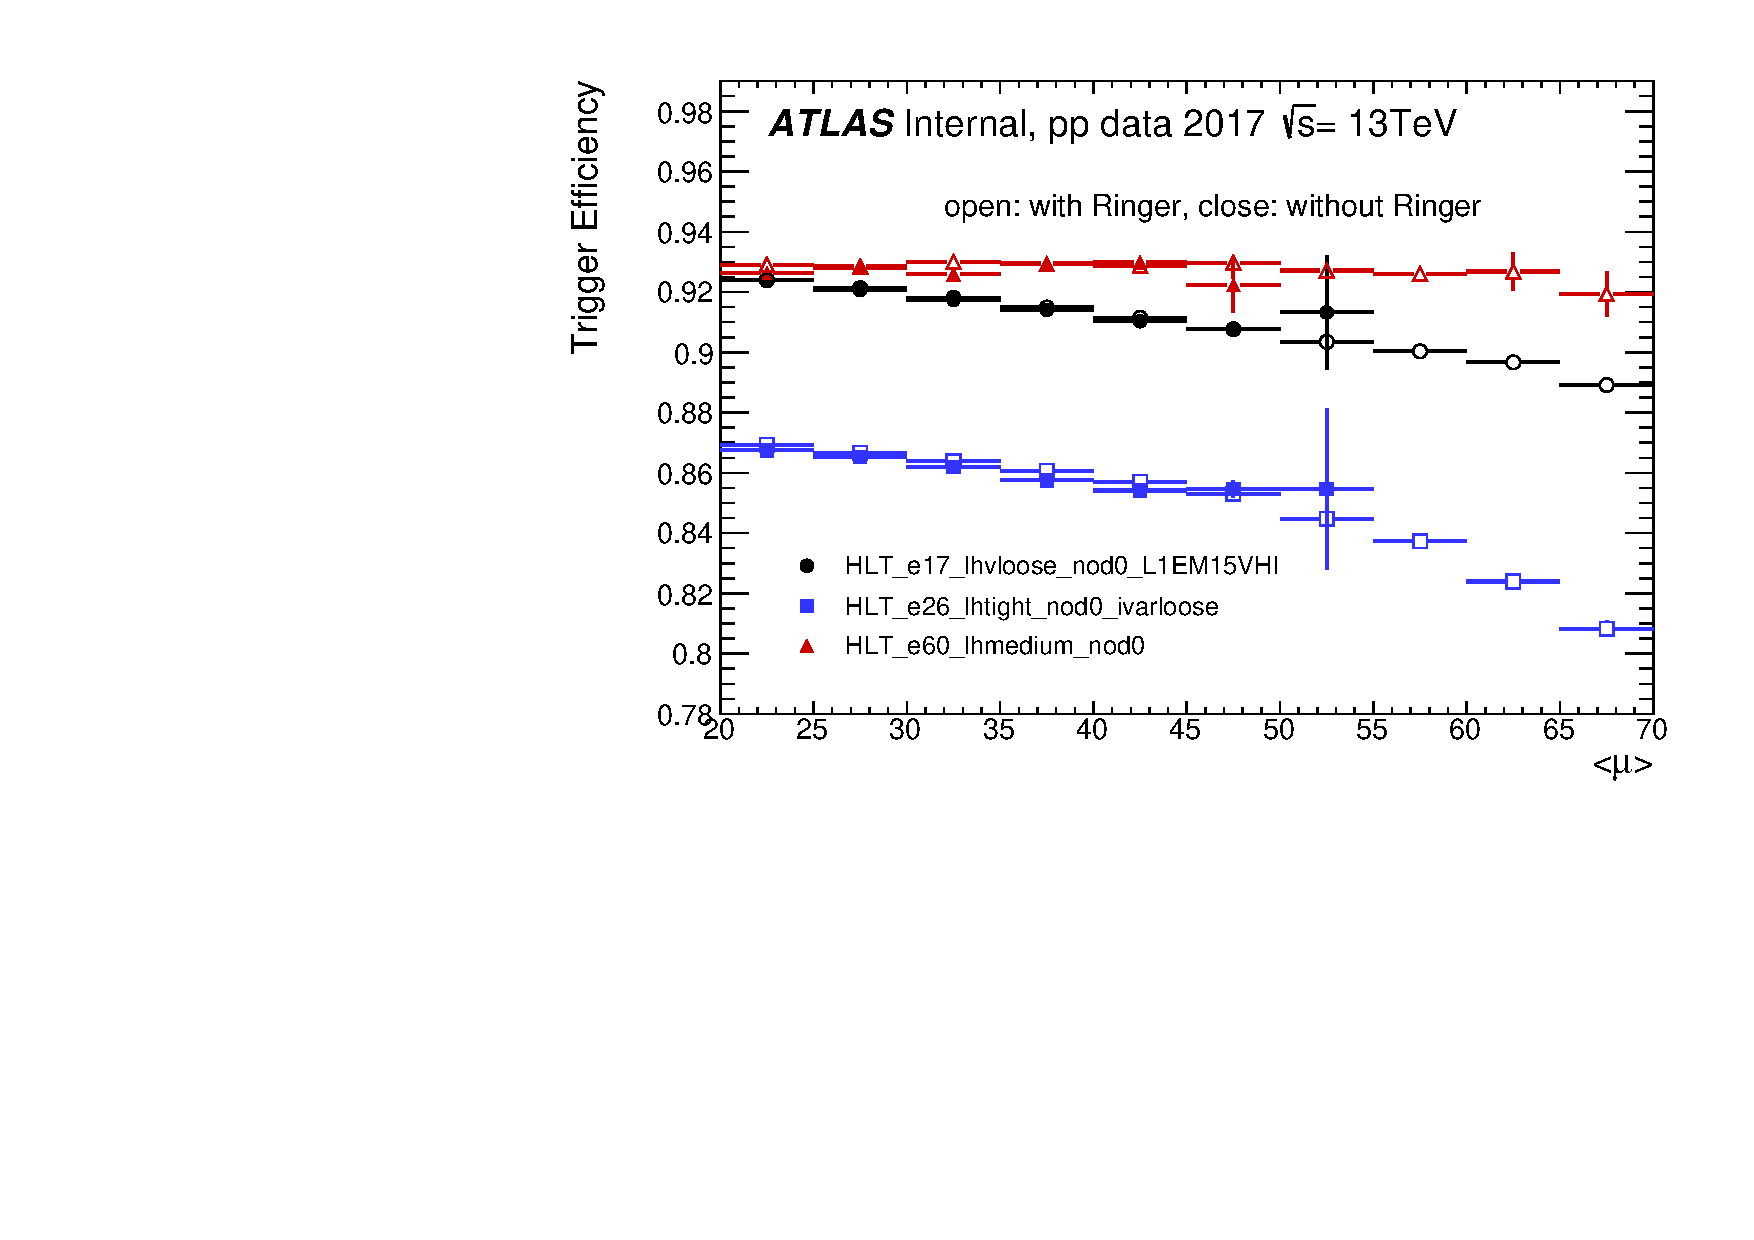
\includegraphics[width=\textwidth]{sections/operation/figures/efficiencies/eff_EGAM1_e17_e26_e60_2017_before_and_after_ts1_mu.pdf}
  \caption{}%
  \end{subfigure}
  %\hfill
  \caption{Efficiency of three single electron triggers as a function of
  \et (a), \eta (b) and \avgmu (c). Open (closed) markers contain
  the efficiency measurements on runs before (after) TS1, thus referring to
  triggers being executed without (with) the \rnn{} algorithm.
  }%
  \label{fig:2017_ts1}
  \end{center}
\end{figure}


By contrasting the behavior of the duplicated trigger using fake electron data,
it becomes clear the power of the \rnn{} algorithm. An overall reduction factor of
the fake rate by 13.75 is achieved. It can be seen in
Figure~\ref{fig:e28_triggers_fake} that the improvement is similar for all
regions in the evaluated variables, particularly interesting when
considering the low \et{} and the end-cap regions.




\begin{figure}[h!tb]
  \begin{center}
  \begin{subfigure}[c]{.48\textwidth}
  \centering
  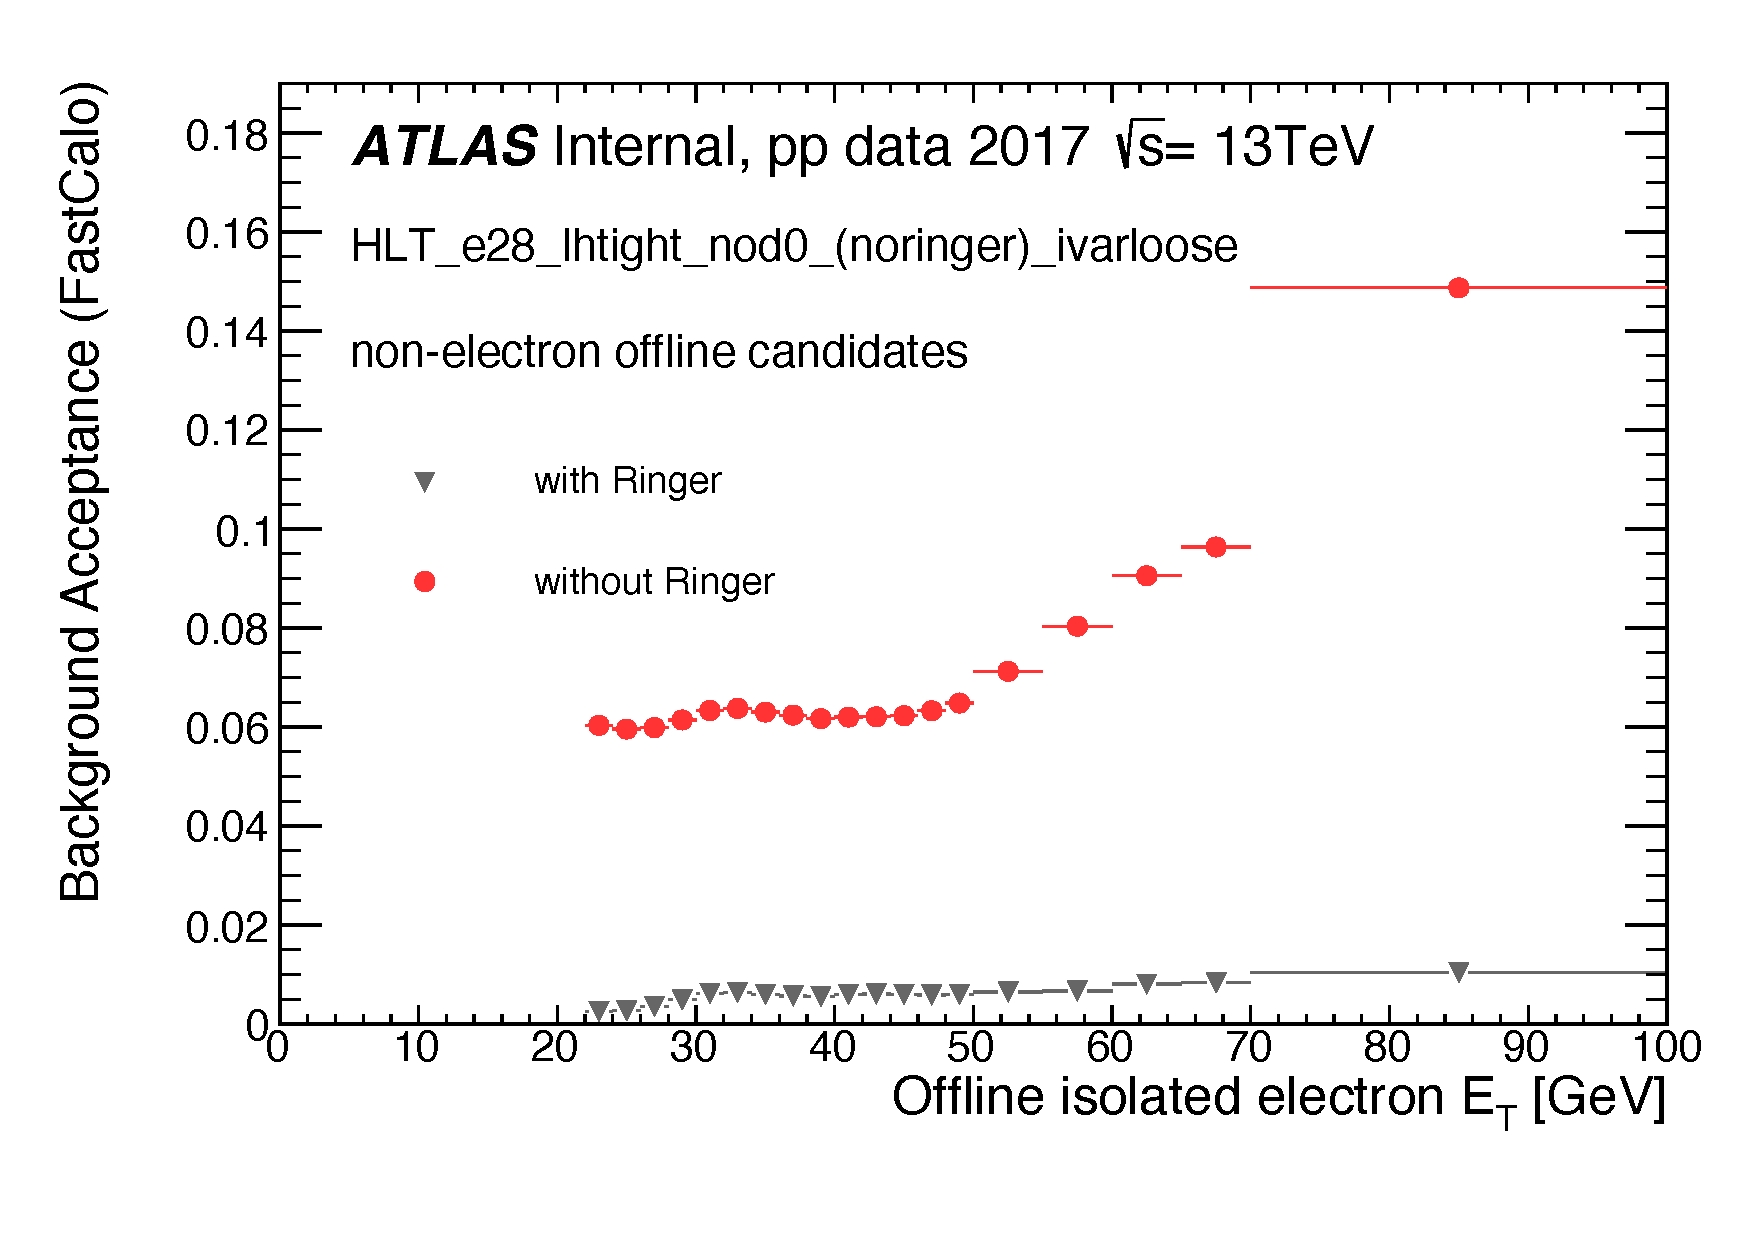
\includegraphics[width=\textwidth]{sections/operation/figures/efficiencies/eff_EGAM7_e28_ringer_and_noringer_2017_after_ts1_L2Calo_et.pdf}
  %\label{fig:e28_comp_et_fake}
  \caption{}
  \end{subfigure}
  \hfill
  %\hspace{0.01\textwidth}
  \begin{subfigure}[c]{.48\textwidth}
  \centering
  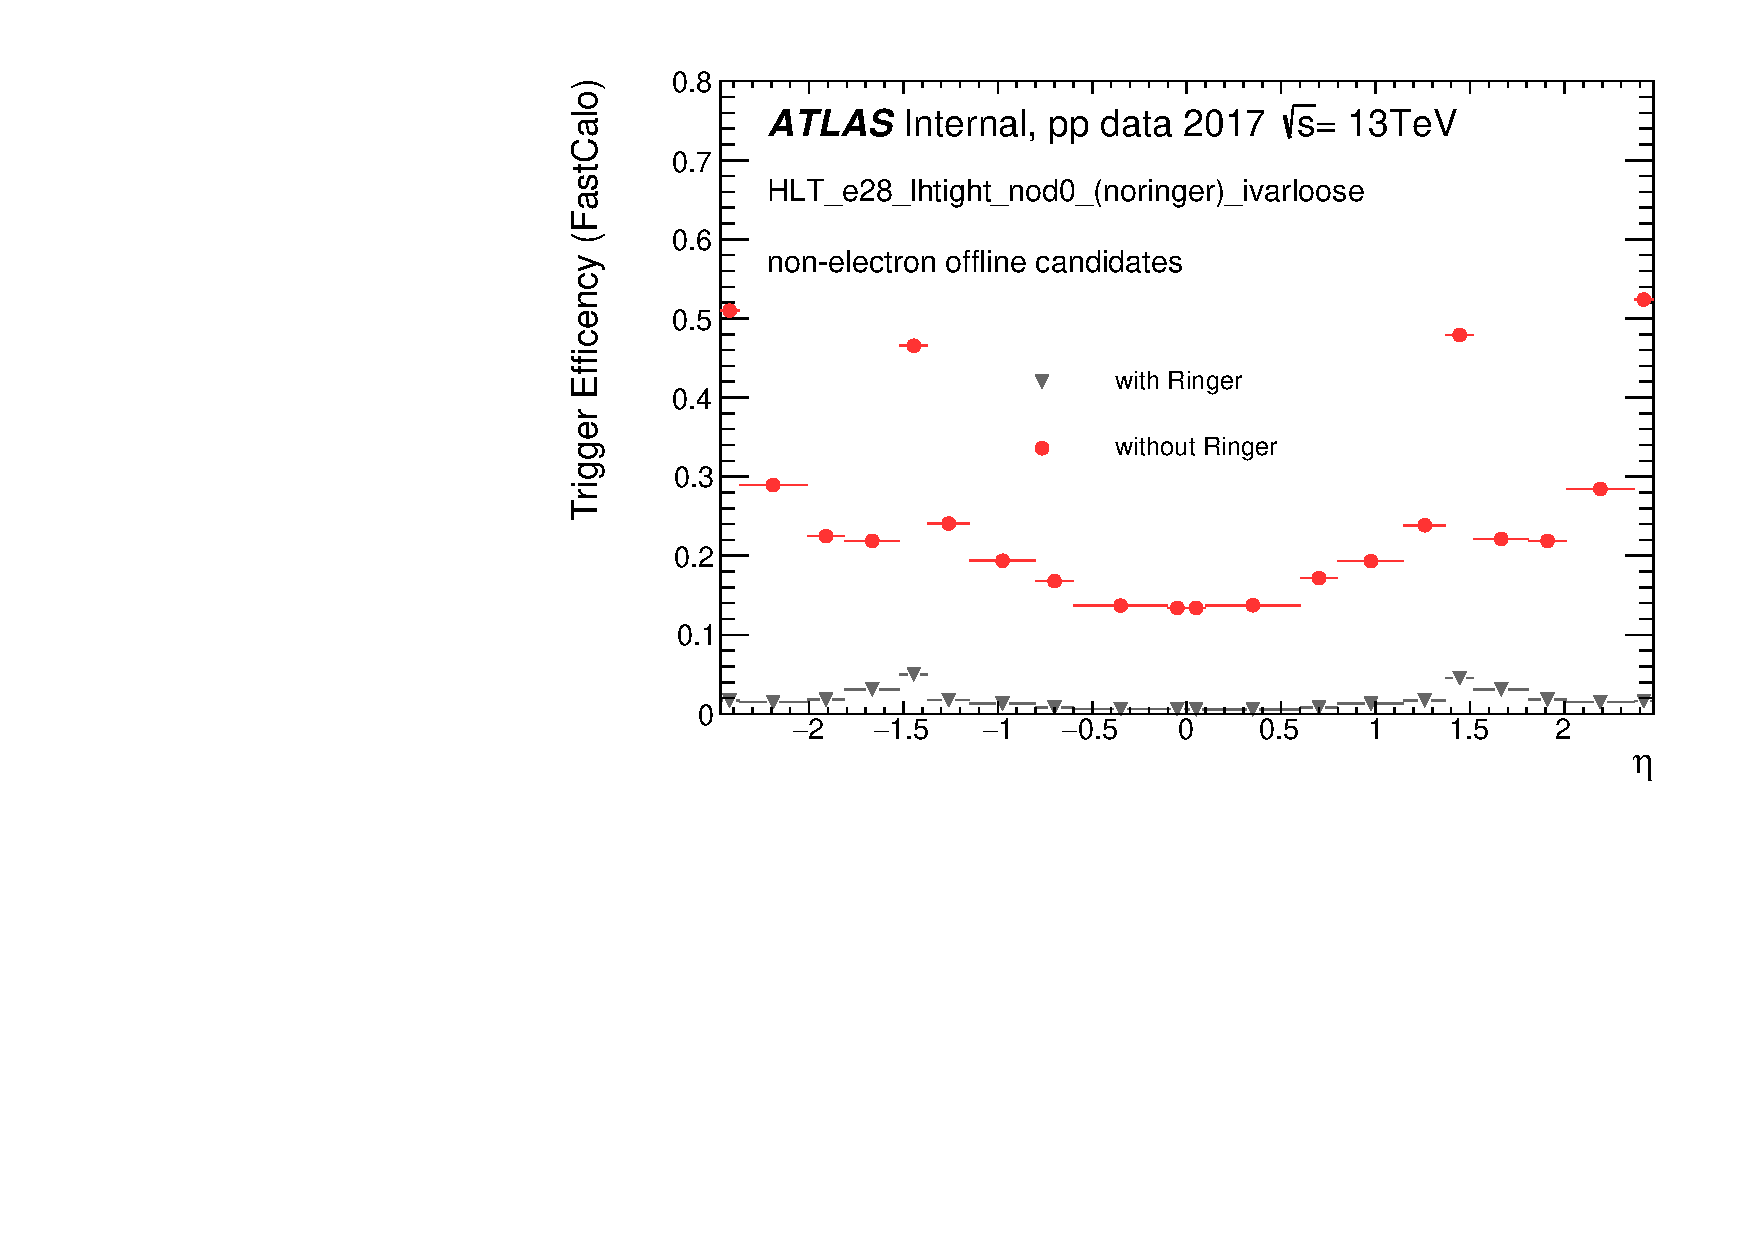
\includegraphics[width=\textwidth]{sections/operation/figures/efficiencies/eff_EGAM7_e28_ringer_and_noringer_2017_after_ts1_L2Calo_eta.pdf}
  %\label{fig:e28_comp_eta_fake}
  \caption{}
  \end{subfigure}\\
  \begin{subfigure}[c]{.48\textwidth}
  \centering
  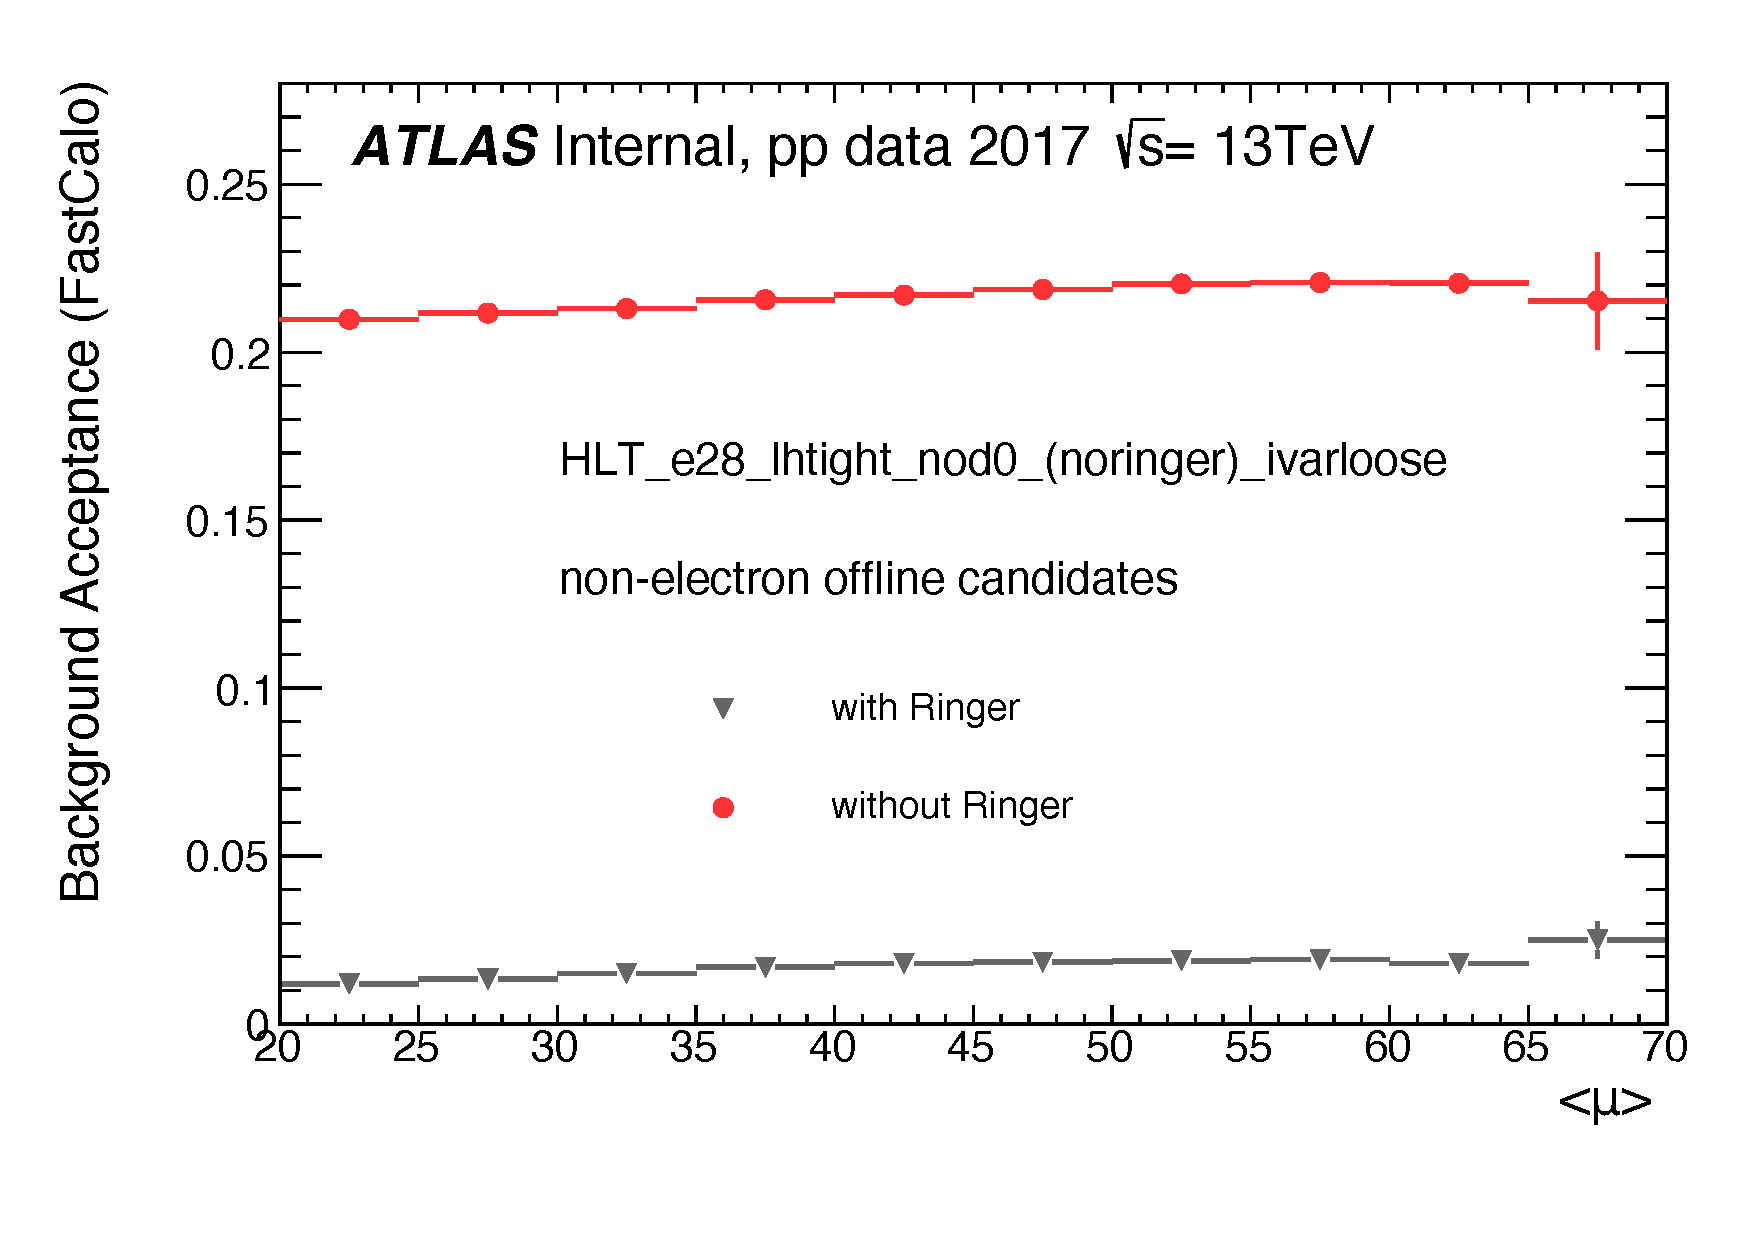
\includegraphics[width=\textwidth]{sections/operation/figures/efficiencies/eff_EGAM7_e28_ringer_and_noringer_2017_after_ts1_L2Calo_mu.pdf}
  %\label{fig:e28_comp_mu_fake}
  \caption{}
  \end{subfigure}
  %\hfill
  \caption{\label{fig:e28_triggers_fake} \fastcalo %\footnotemark{} 
  fake electron efficiency as a function of \et (a), \eta (b) and \avgmu (c) for the
  duplicated single electron trigger requiring $\et > \SI{28}{\GeV}$ and \tight
  selection with and without the \rnn{} algorithm. Efficiencies are measured
  employing 2017 data collected after TS1.}%
  
  \end{center}
\end{figure}


%\footnotetext{Actually, Figure~\ref{fig:e28_triggers_fake} shows
%\fastelectron efficiency that is nearly the same as the \fastcalo.  \fastcalo
%efficiencies could not be retrieved due to limitations in the software.}



Besides the capability of improving early fake rejection, the usage of the
\rnn{} also contributed to reduce the final fake rate
(Figure~\ref{fig:e28_triggers_fake_hlt}) by a factor of 2, mostly coming from
the end-cap and crack regions. %This fake rate reduction when measured with
%respect to the offline electron selection does not seem to have impacted in the
%output rate (see Appendix~\ref{ssec:primary_rate_wrt_luminosity})\footnote{This
%  can provide some indication that measuring background efficiencies with
%respect to the offline may not be the best approach.}, but may have
%contributed to reduce signal contamination in physics analyses.

\begin{figure}[h!tb]
\begin{center}
\begin{subfigure}[c]{.48\textwidth}
\centering
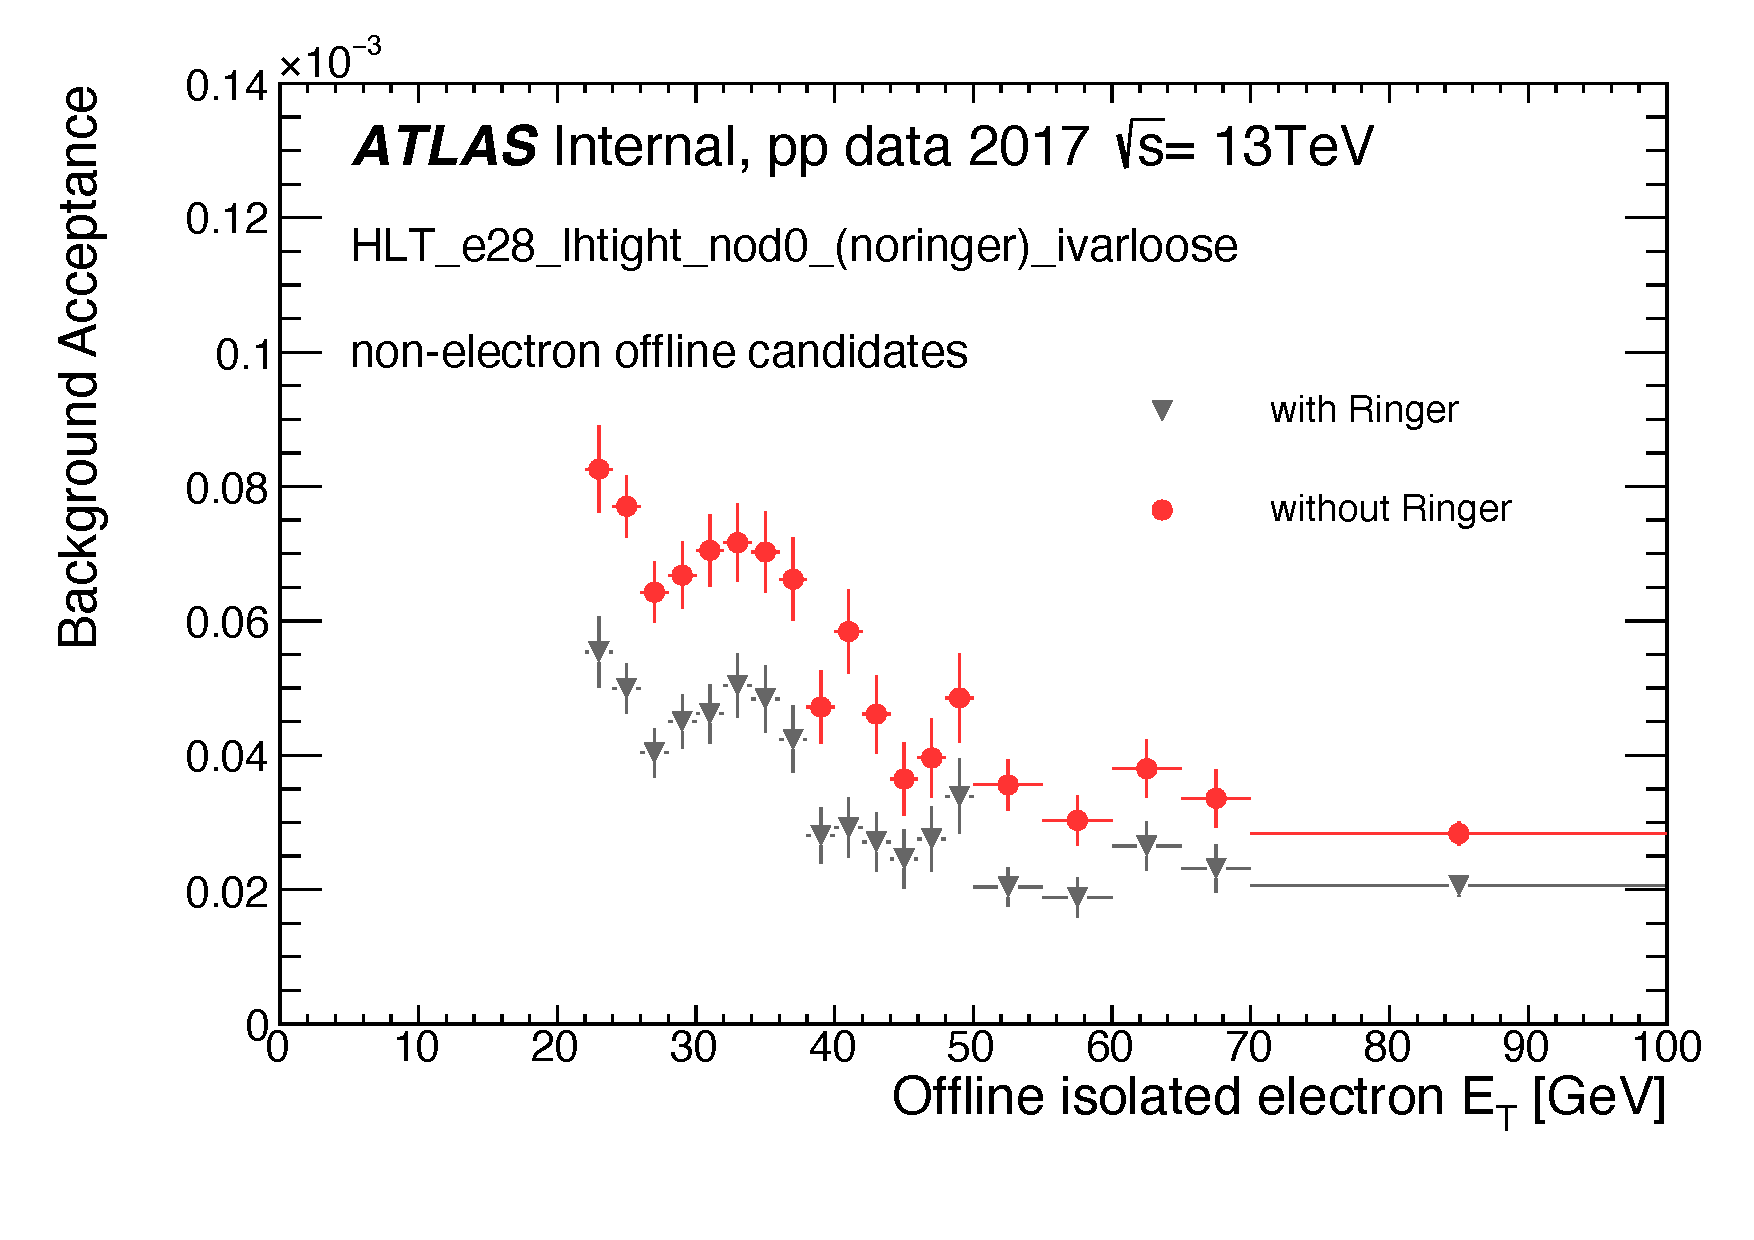
\includegraphics[width=\textwidth]{sections/operation/figures/efficiencies/eff_EGAM7_e28_ringer_and_noringer_2017_after_ts1_et.pdf}
\caption{}
\end{subfigure}
\hfill
%\hspace{0.01\textwidth}
\begin{subfigure}[c]{.48\textwidth}
\centering
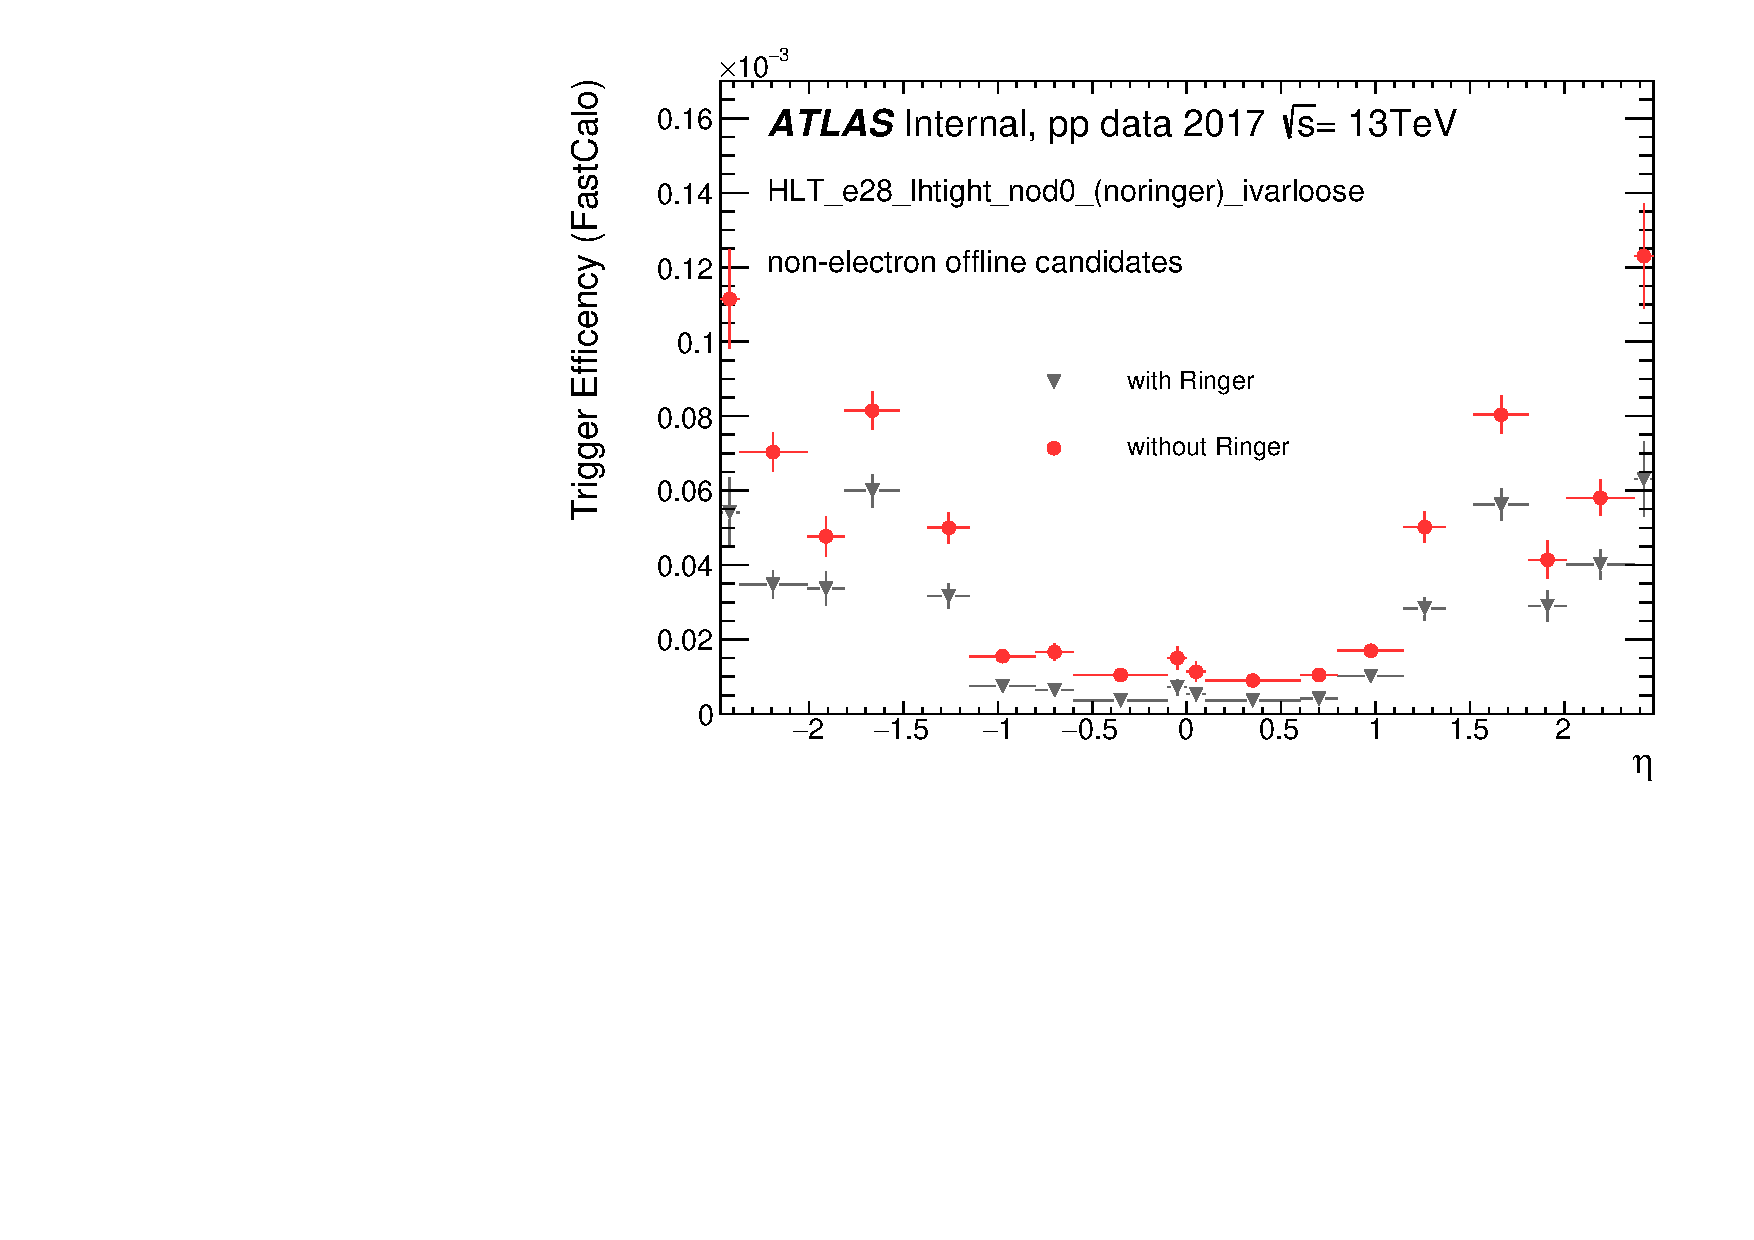
\includegraphics[width=\textwidth]{sections/operation/figures/efficiencies/eff_EGAM7_e28_ringer_and_noringer_2017_after_ts1_eta.pdf}
\caption{}
\end{subfigure} \\
\begin{subfigure}[c]{.48\textwidth}
\centering
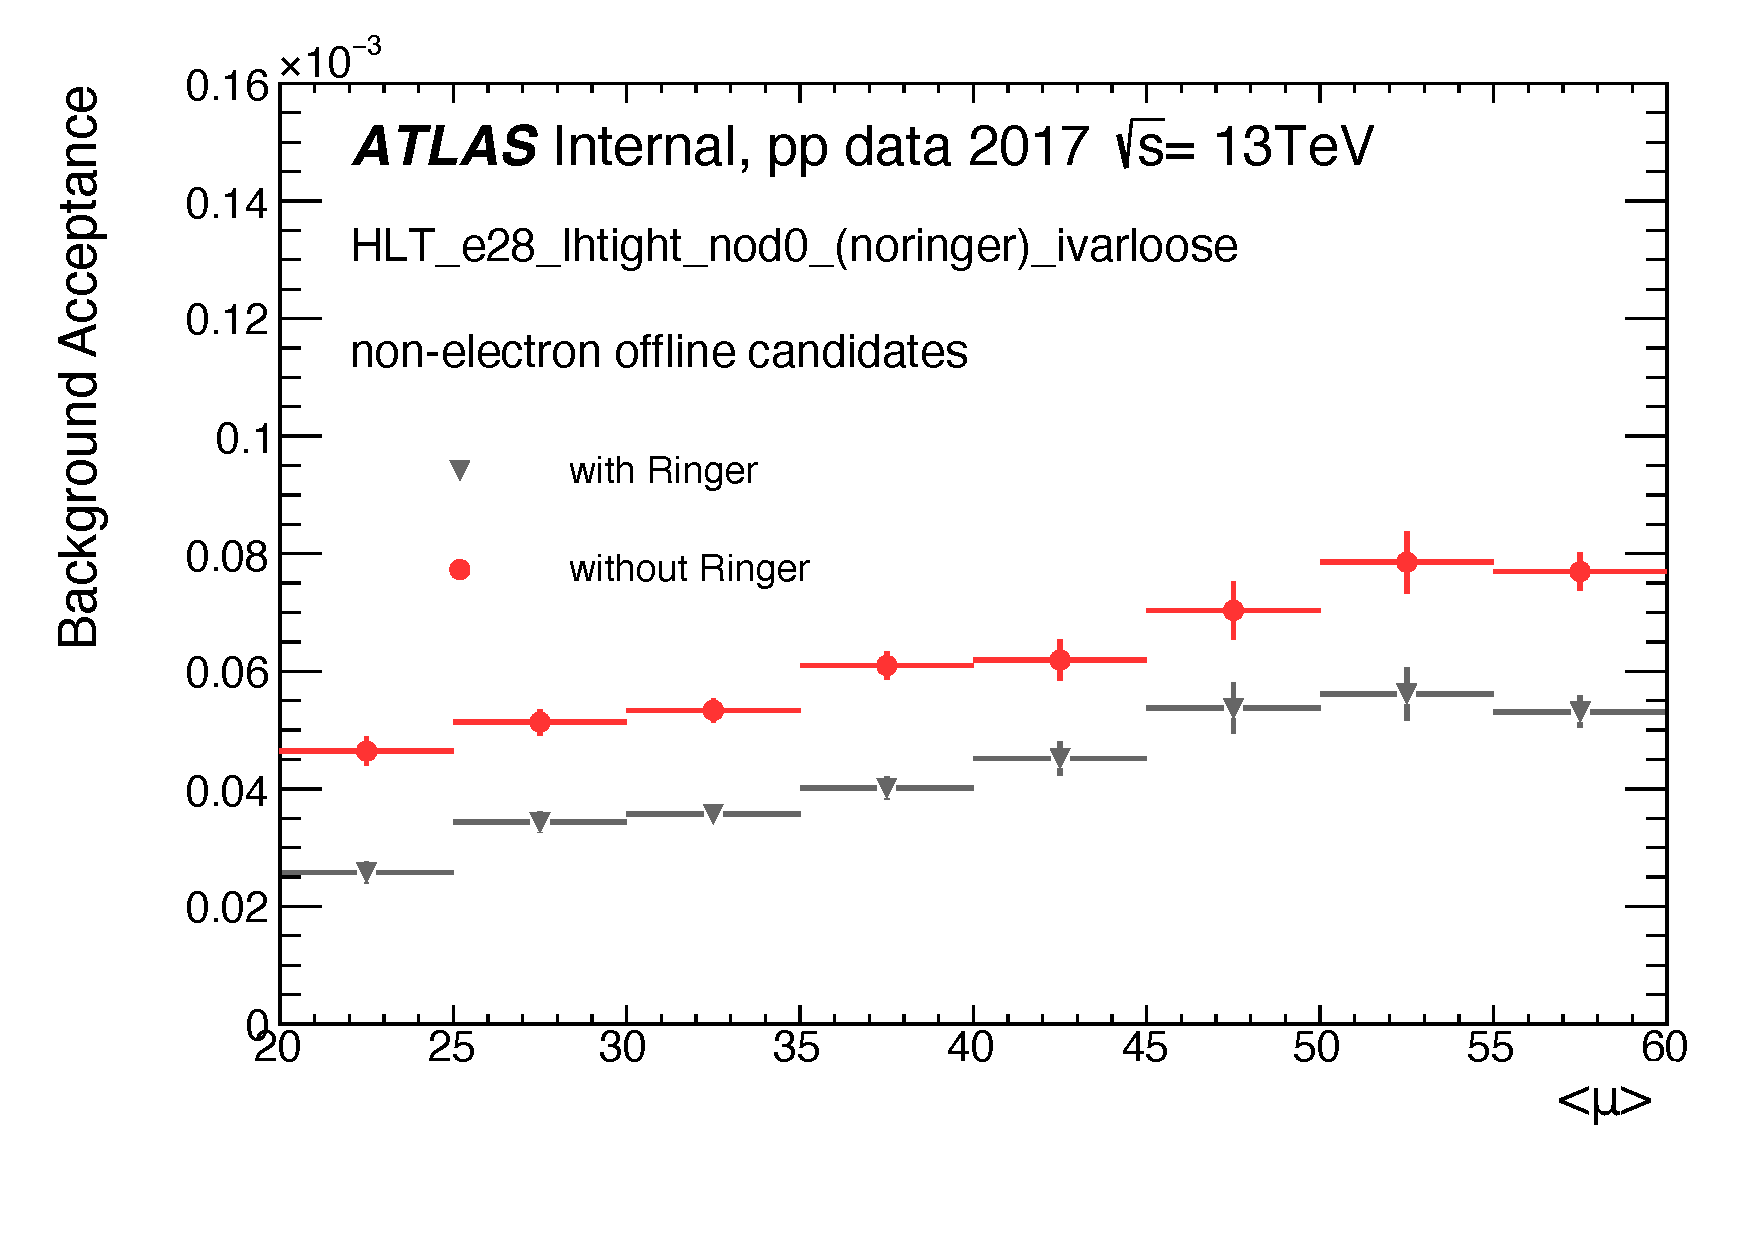
\includegraphics[width=\textwidth]{sections/operation/figures/efficiencies/eff_EGAM7_e28_ringer_and_noringer_2017_after_ts1_mu.pdf}
\caption{}
\end{subfigure}
\caption{HLT fake electron efficiency as a function of \et (a), \eta (b) and
\avgmu (c) for the duplicated single electron trigger requiring $\et >
\SI{28}{\GeV}$ and \tight selection with and without the \rnn{} algorithm.
Efficiencies are measured employing 2017 data collected after TS1.}%
\label{fig:e28_triggers_fake_hlt}
\end{center}
\end{figure}

\FloatBarrier

\section{2018 Operation}\label{ssec:2018_ringer_operation}

In 2018, the \rnn{} operated with a new tune based on collision data
(Section~\ref{ssec:2018}). It was also the case for the final HLT
selection\footnote{One exception was the \medium{} selection, where the HLT
likelihood selection operated in 2018 with the same 2017 tune.}. For the
\textcolor{red}{lowest-transverse energy-threshold}
%lowest-energy-threshold 
unprescaled trigger, an efficiency
improvement of at least one percentage point in central value is observed when
comparing both periods, resulting from a better operation in all selection
steps, but, in particular,
\textcolor{red}{this is due to improvements from the likelihood tunes in the period.}
%due to the improvement of the likelihood tunes.
Figure~\ref{fig:primary_triggers_comp_2018} shows that this improvement is
coming mostly from electrons around \SI{40}{\GeV} in the center of ATLAS.\@ It
also shows the improvement with respect to \avgmu at higher pile-up conditions
as a result of the larger correction range. Despite maintaining high electron efficiency, a reduction factor up to 1.69 in the \fastcalo{} fake rate was obtained.

%The remaining primary triggers are
%shown in Figure~\ref{fig:primary_triggers_comp_e60_e140_2018}, where efficiency
%is mostly kept unchanged. For the e60\_lhmedium\_nod0 trigger, the lower
%efficiency in the crack region is due to \licalo. Although the electron
%efficiency was maintained high, Table~\ref{tab:2018_fake_rate} shows a reduction
%in the \fastcalo{} fake rate in 2018.  It may count with contributions from both
%the less stringent data taking conditions during 2018 and the training of neural
%networks with collision data.

% TODO Plot of fake rate during vs 2017 for fakes.
% TODO Plot e26, e60 etc would be better using data during the commisioning
% stages.

\begin{figure}[h!tb]
\centering
\begin{subfigure}[c]{.48\textwidth}
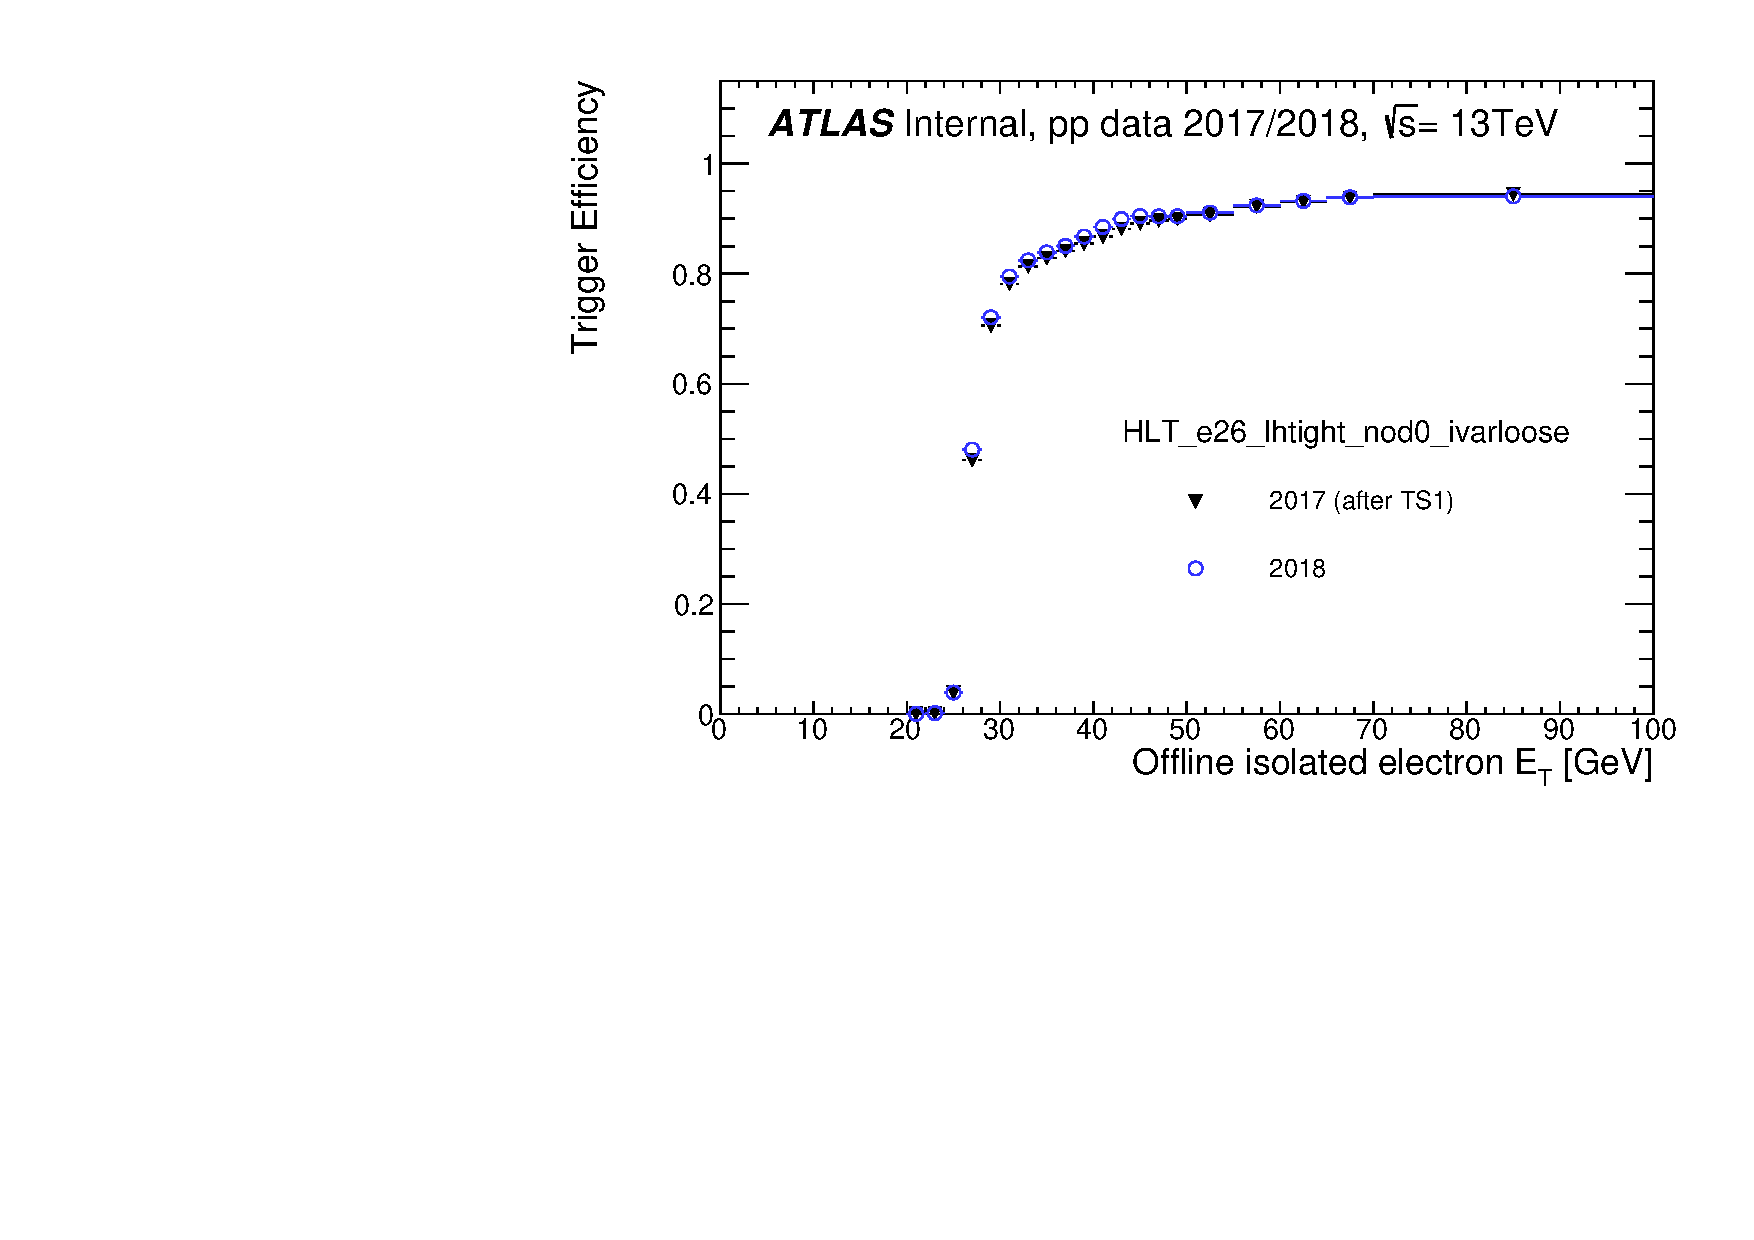
\includegraphics[width=\textwidth]{sections/operation/figures/efficiencies/eff_EGAM1_e26_lhtight_nod0_ivarloose_2017_after_ts1_and_2018_et.pdf}
\caption{}
\end{subfigure}
\hfill
%\hspace{0.01\textwidth}
\begin{subfigure}[c]{.48\textwidth}
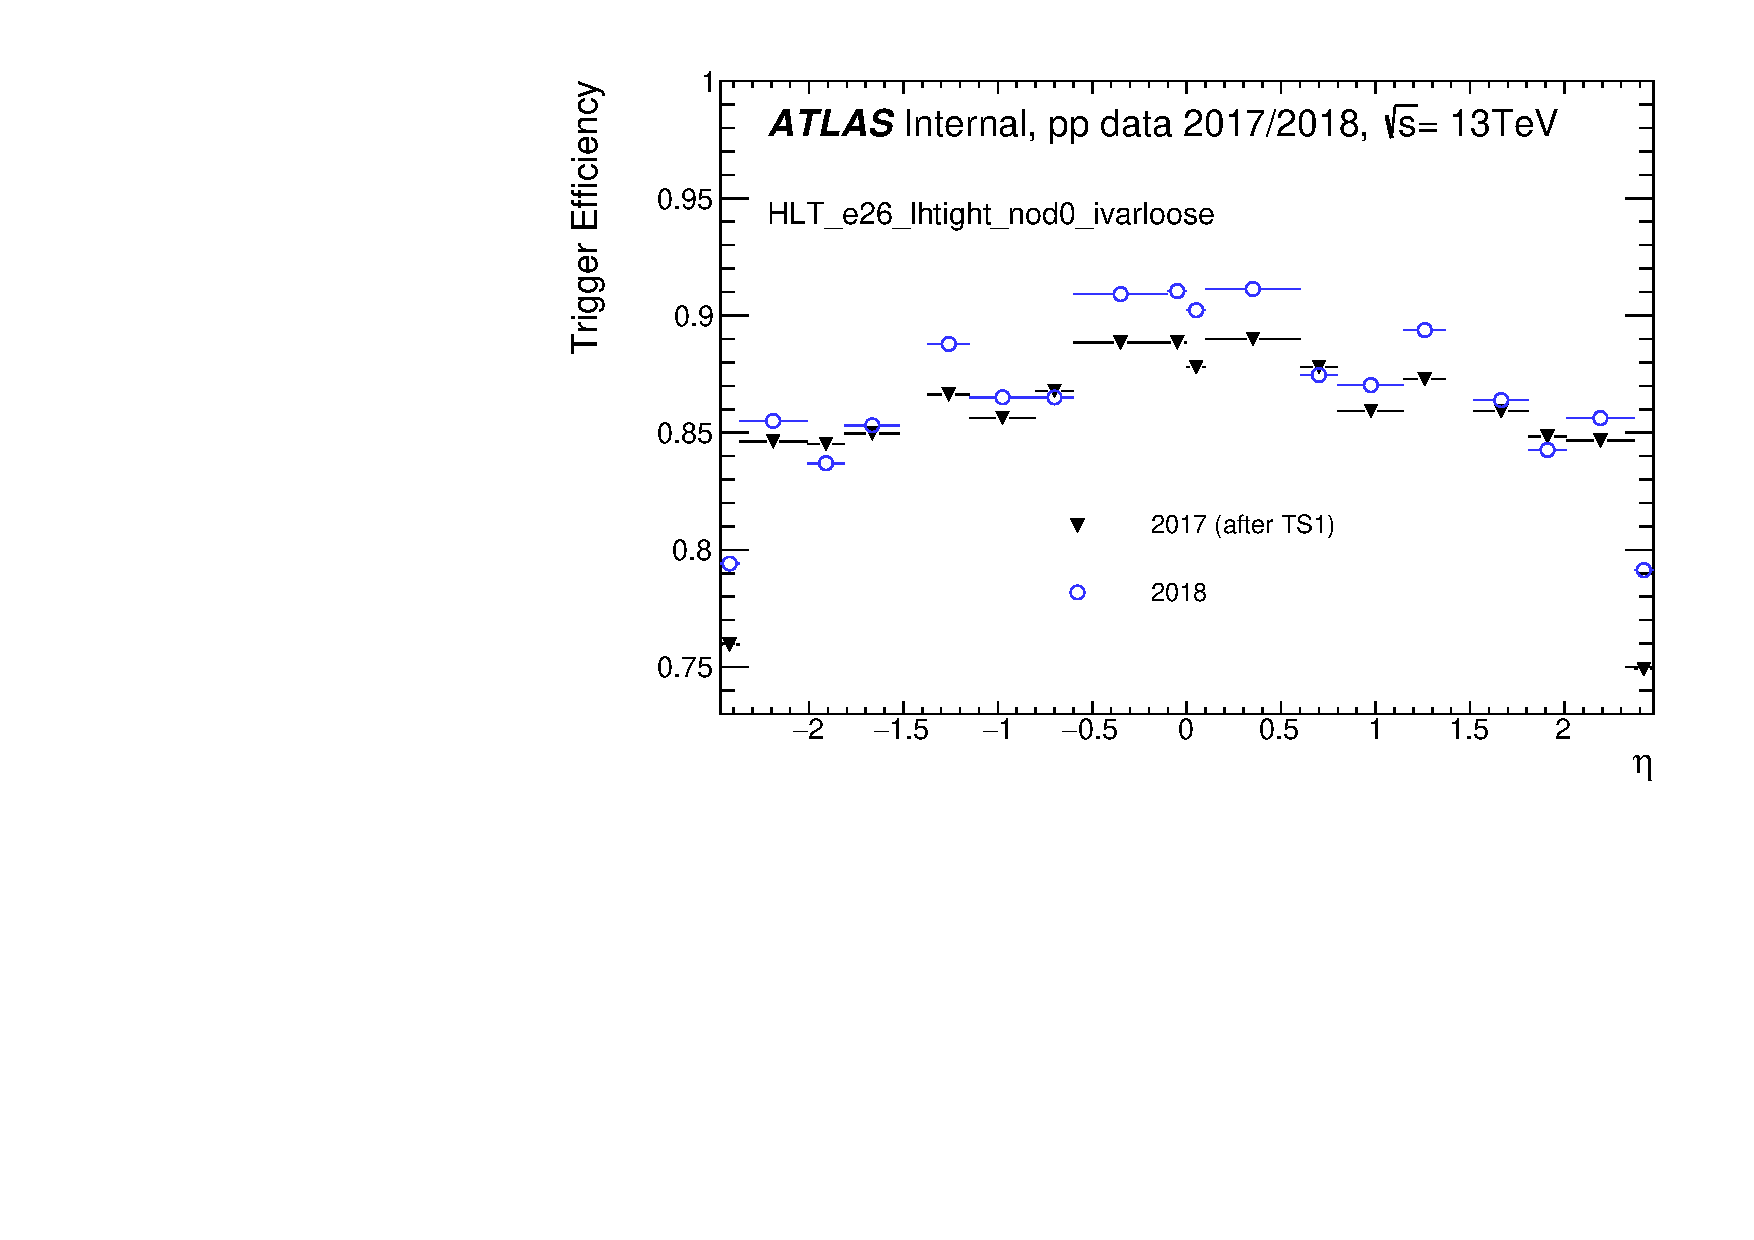
\includegraphics[width=\textwidth]{sections/operation/figures/efficiencies/eff_EGAM1_e26_lhtight_nod0_ivarloose_2017_after_ts1_and_2018_eta.pdf}
\caption{}
\end{subfigure} \\
\begin{subfigure}[c]{.48\textwidth}
\centering
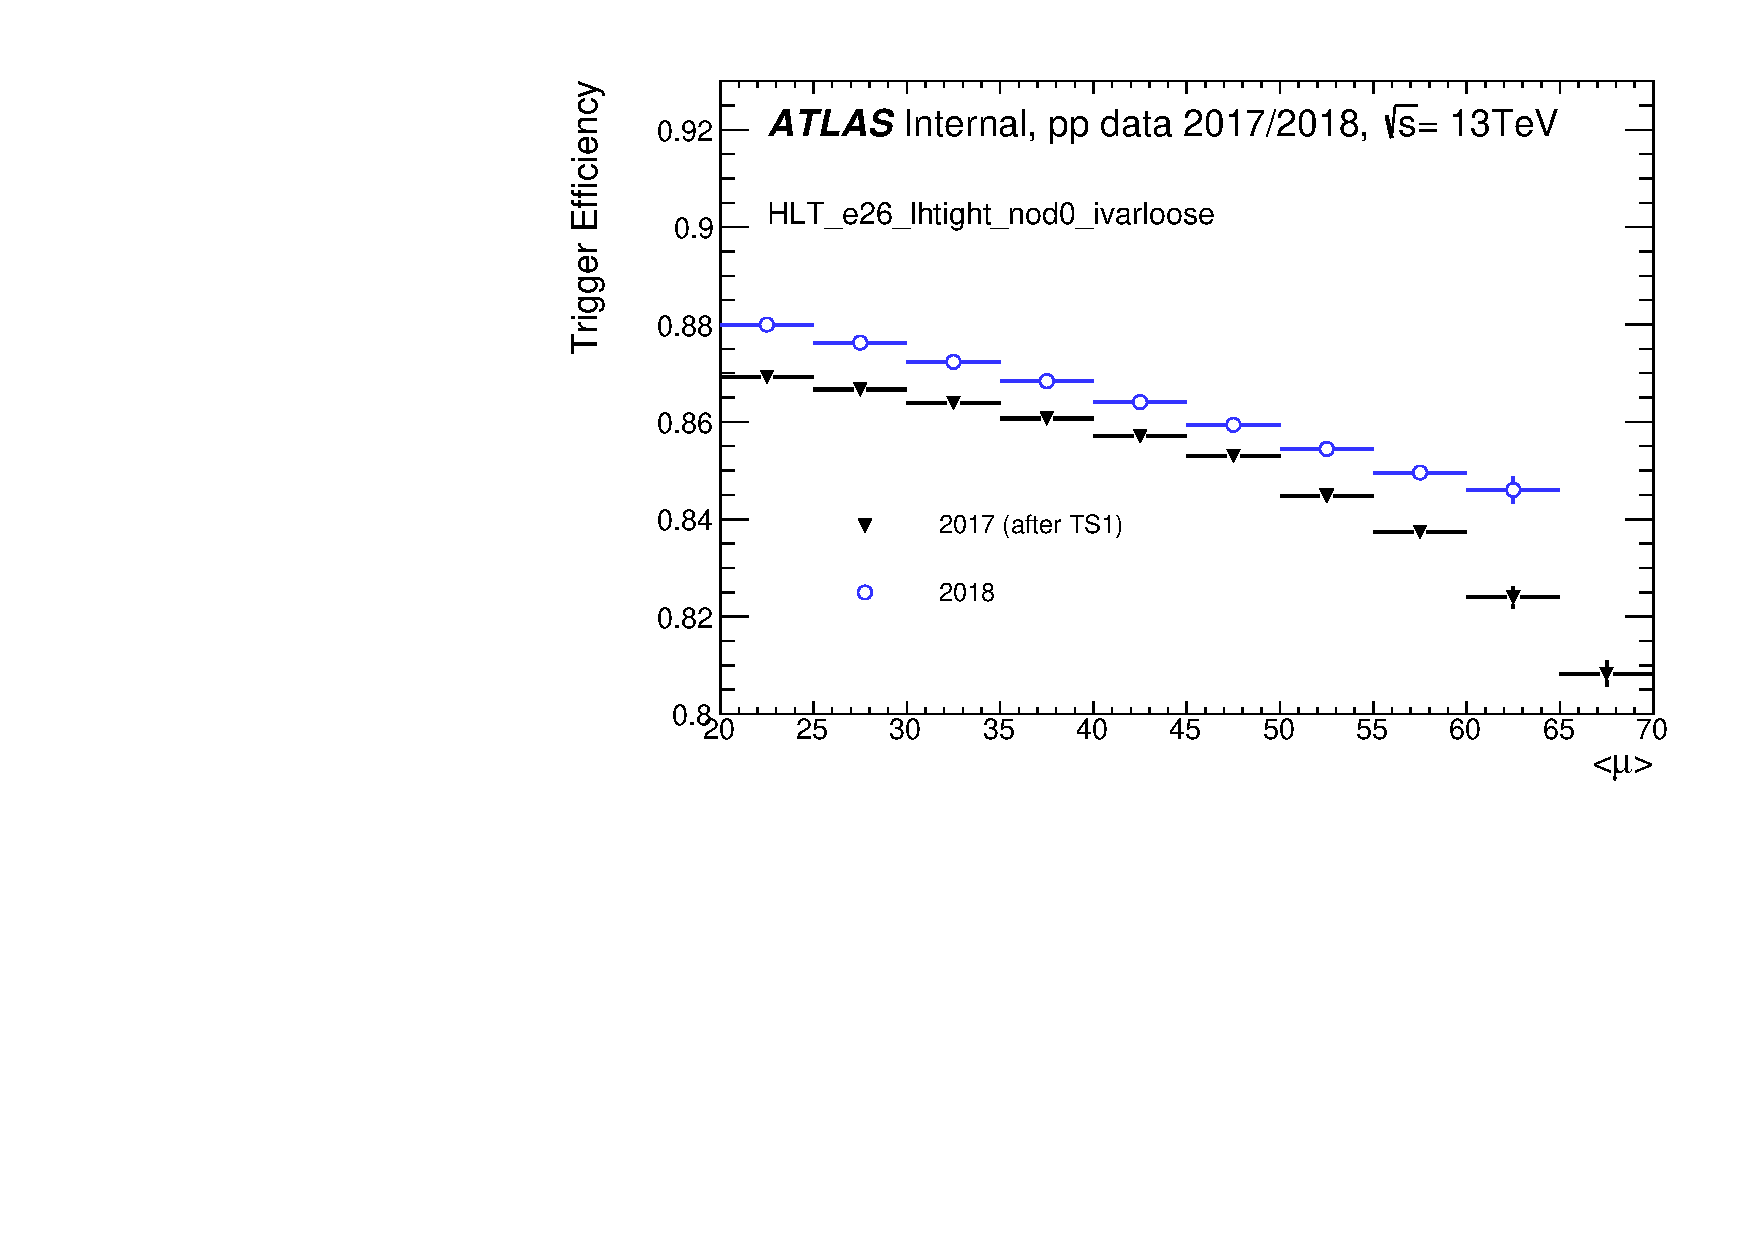
\includegraphics[width=\textwidth]{sections/operation/figures/efficiencies/eff_EGAM1_e26_lhtight_nod0_ivarloose_2017_after_ts1_and_2018_mu.pdf}
\caption{}
\end{subfigure}
\caption{\label{fig:primary_triggers_comp_2018}HLT efficiency of
lowest-energy-threshold unprescaled single electron trigger as a function of
\et (a), \eta (b) and \avgmu (c). Open (closed) markers contain the efficiency
measurements on 2017 (2018) runs.}
\end{figure}

\begin{comment}
\begin{figure}[h!tb]
\centering
\begin{subfigure}[c]{.48\textwidth}
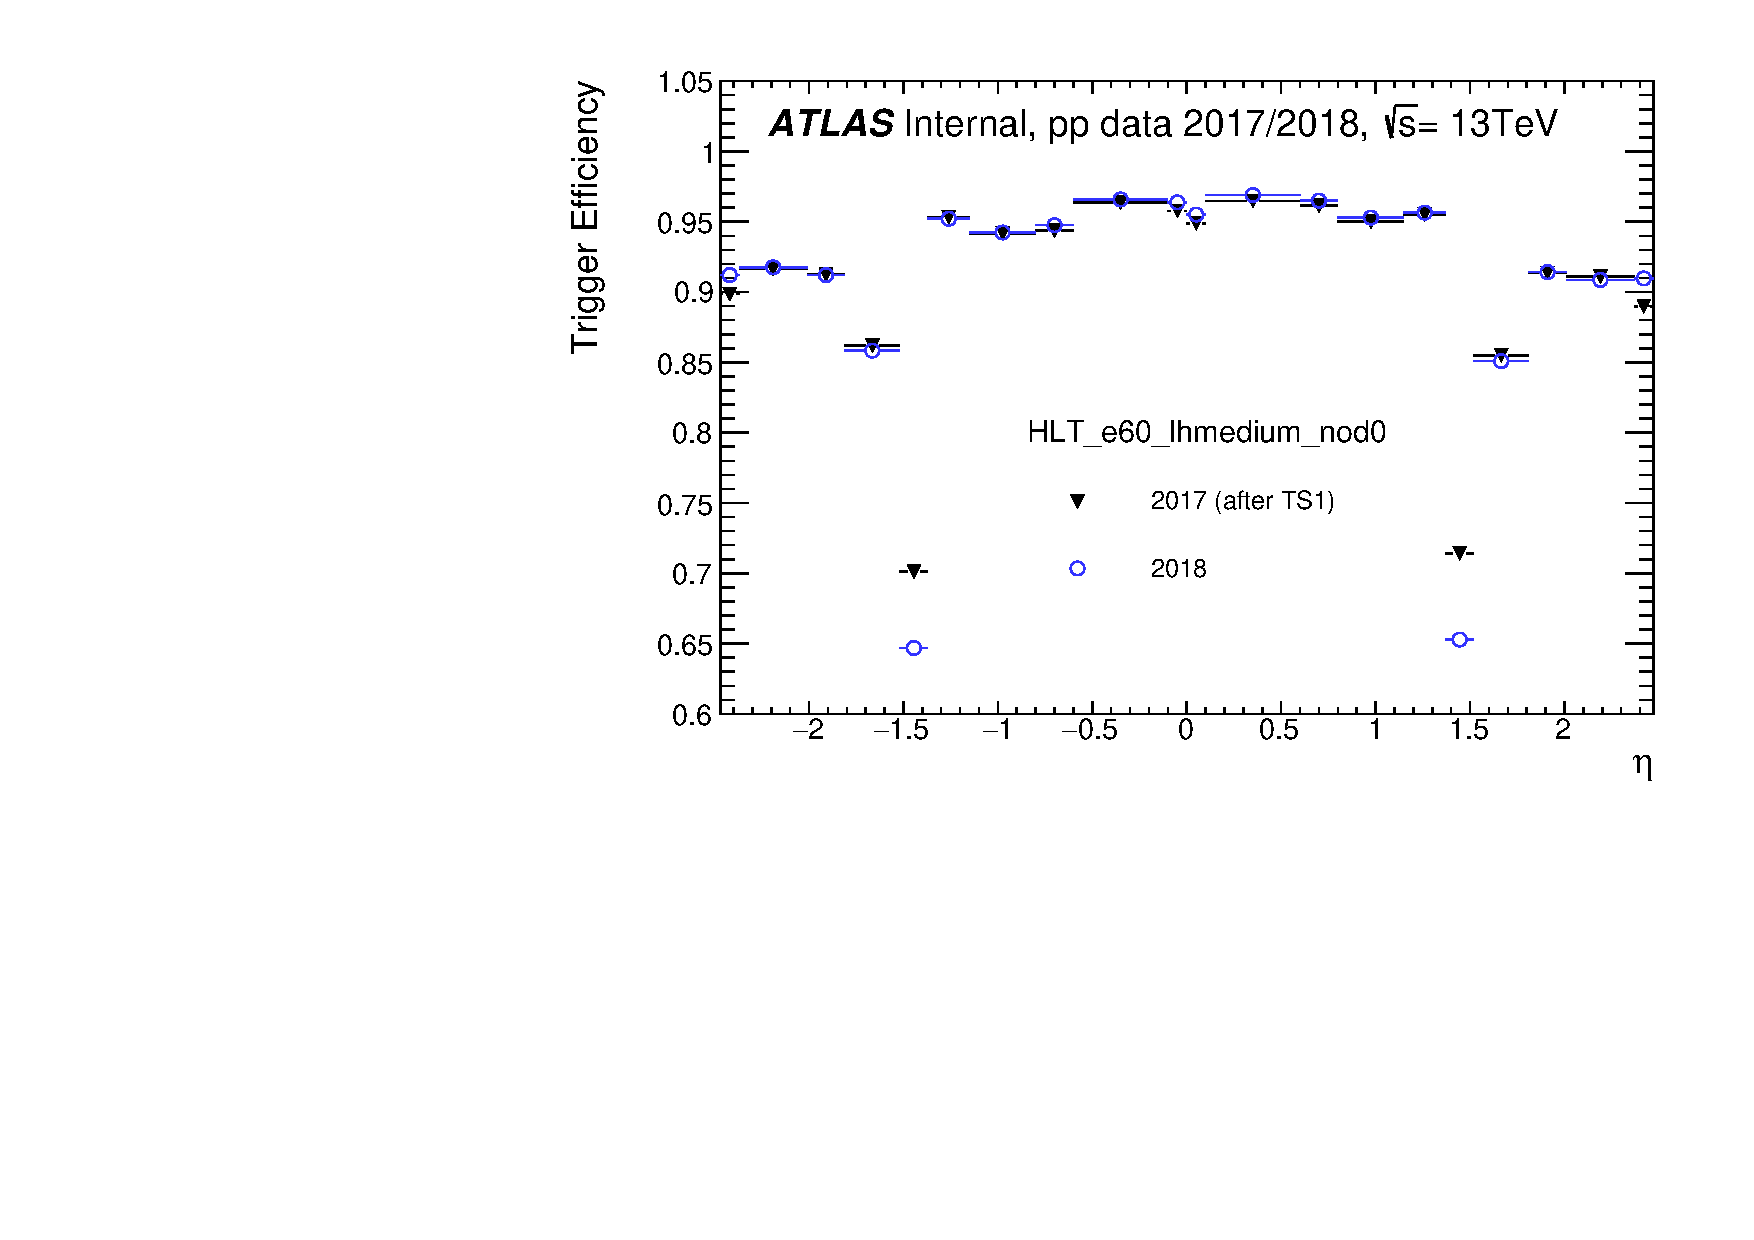
\includegraphics[width=\textwidth]{sections/operation/figures/efficiencies/eff_EGAM1_e60_lhmedium_nod0_L1EM24VHI_2017_after_ts1_and_2018_eta.pdf}
\caption{}
\end{subfigure}
\hfill
%\hspace{0.01\textwidth}
\begin{subfigure}[c]{.48\textwidth}
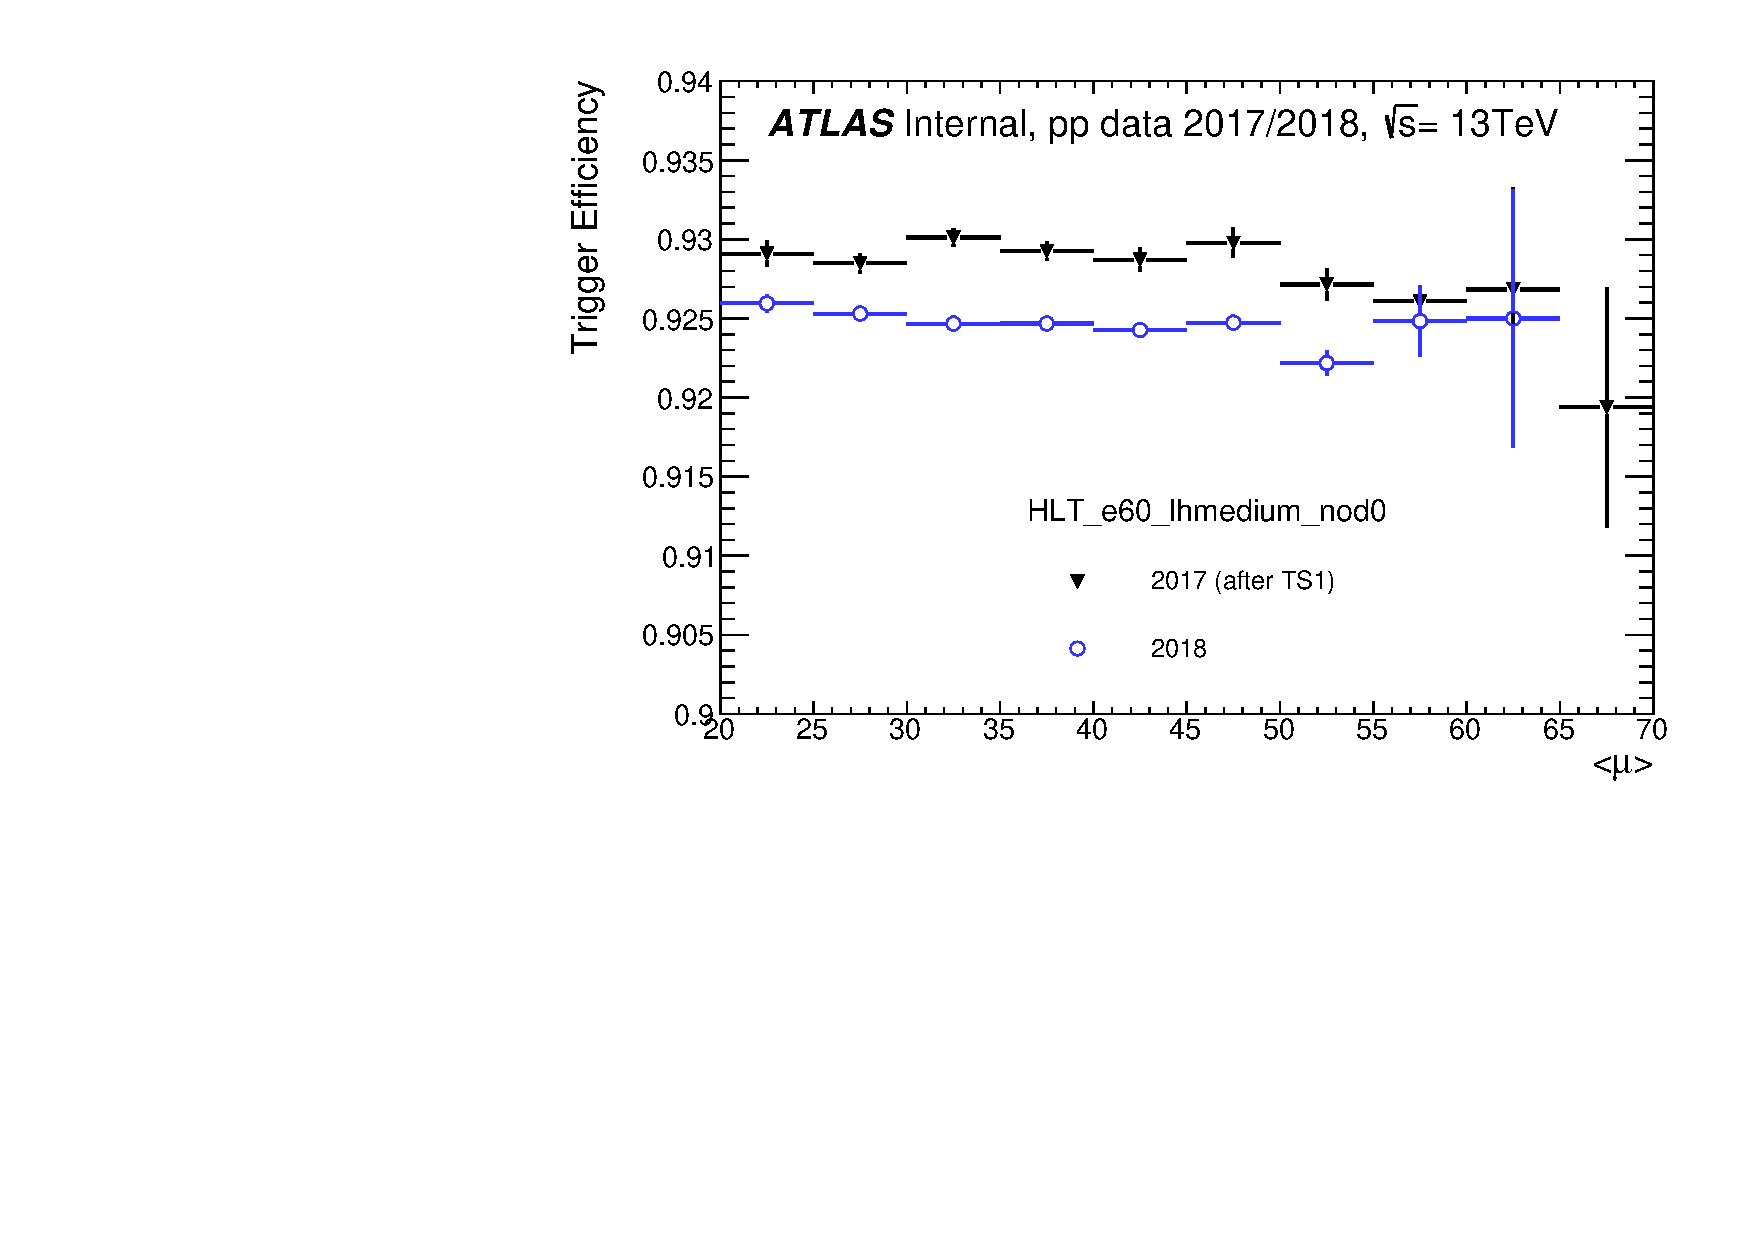
\includegraphics[width=\textwidth]{sections/operation/figures/efficiencies/eff_EGAM1_e60_lhmedium_nod0_L1EM24VHI_2017_after_ts1_and_2018_mu.pdf}
\caption{}
\end{subfigure} \\
\begin{subfigure}[c]{.48\textwidth}
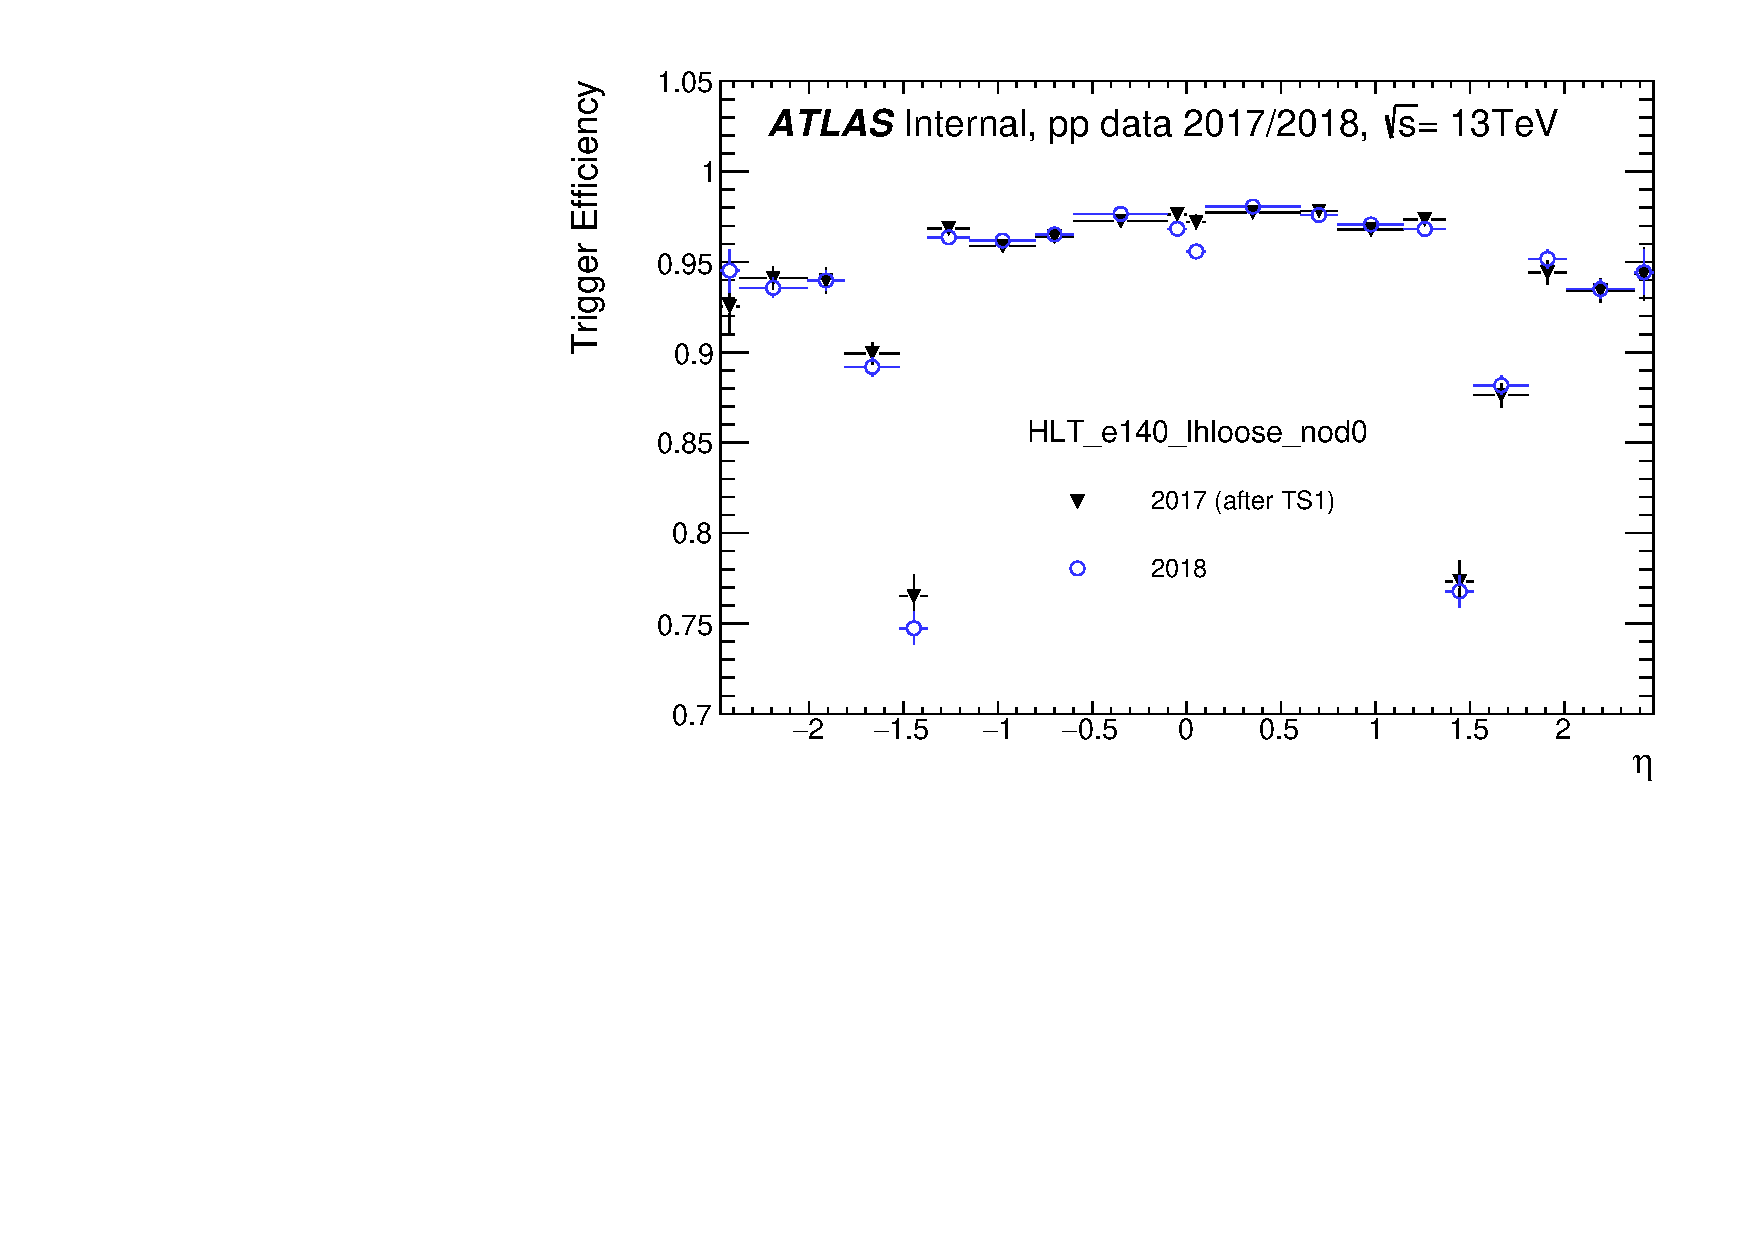
\includegraphics[width=\textwidth]{sections/operation/figures/efficiencies/eff_EGAM1_e140_lhloose_nod0_L1EM24VHI_2017_after_ts1_and_2018_eta.pdf}
\caption{}
\end{subfigure}
\hfill
%\hspace{0.01\textwidth}
\begin{subfigure}[c]{.48\textwidth}
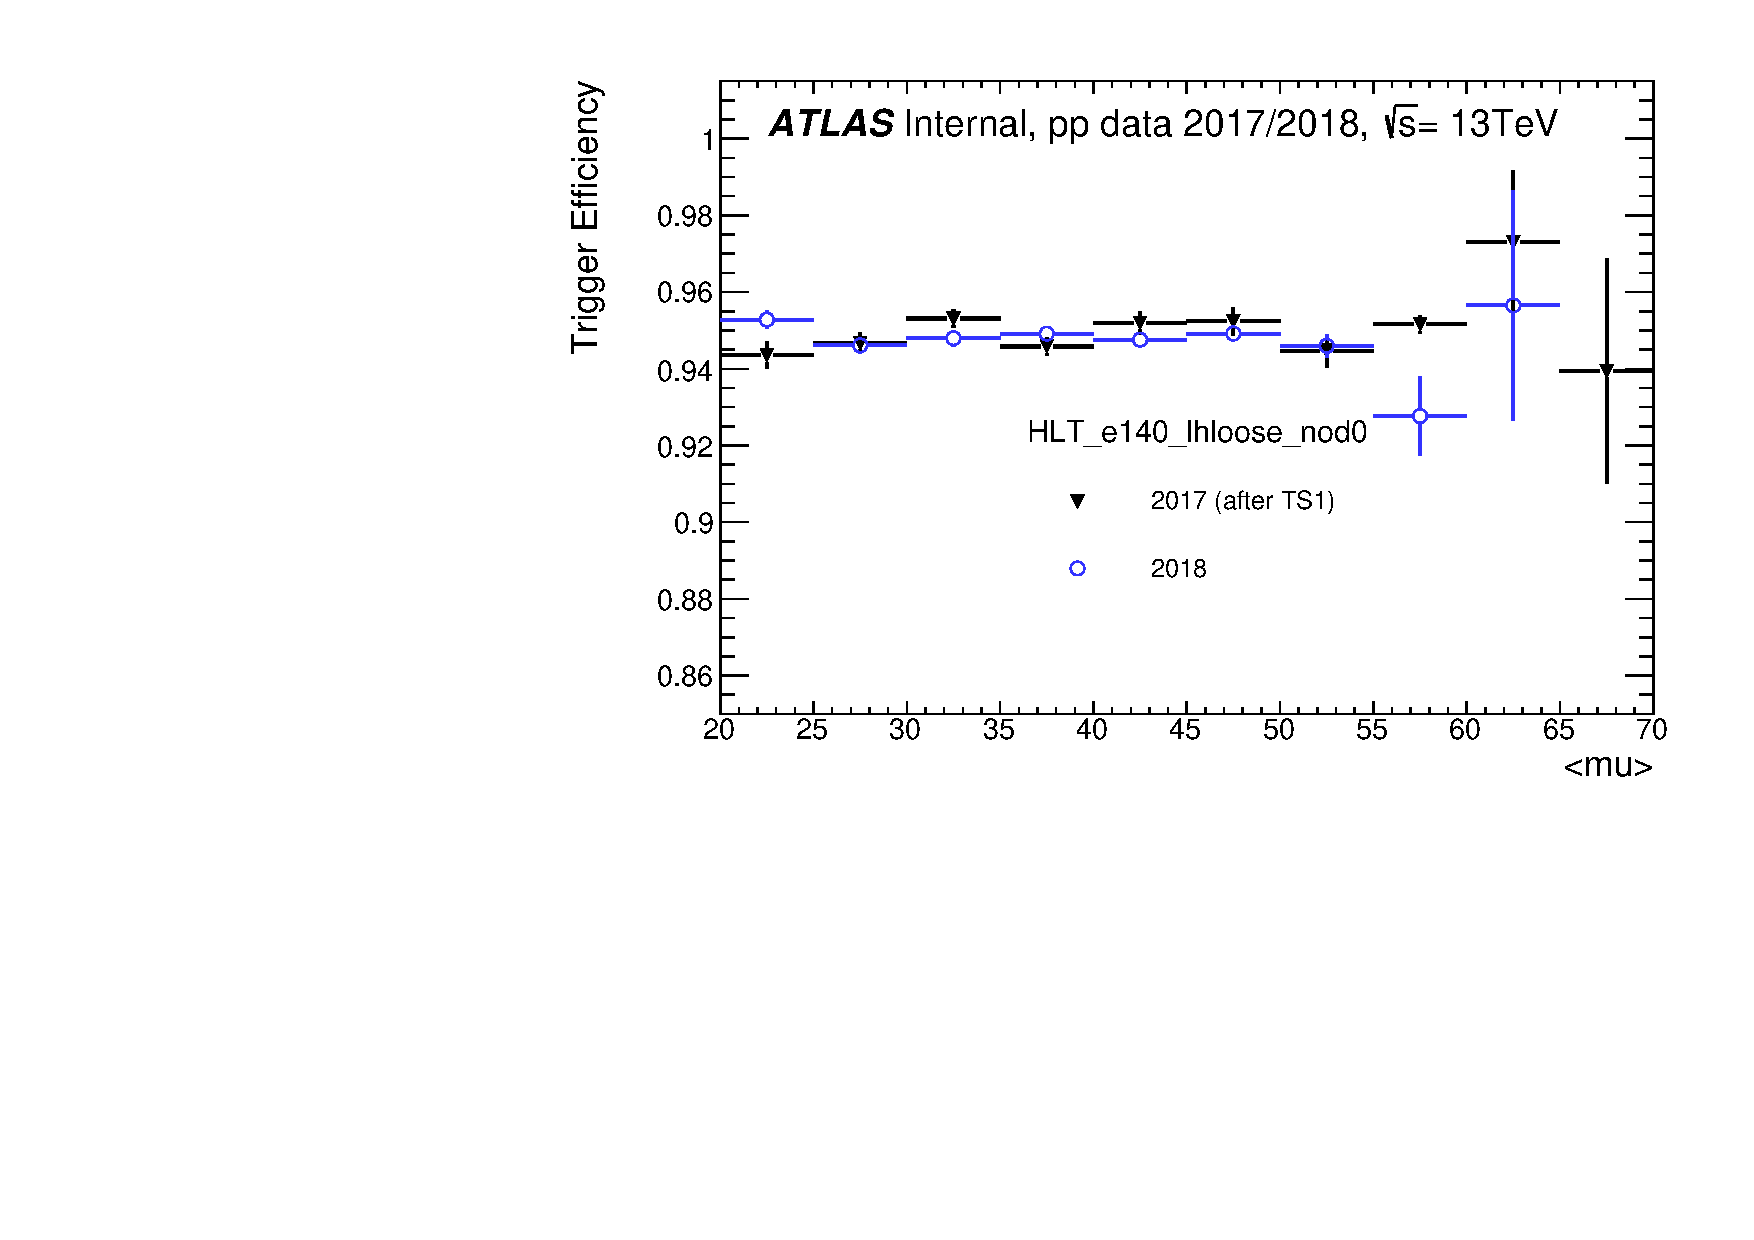
\includegraphics[width=\textwidth]{sections/operation/figures/efficiencies/eff_EGAM1_e140_lhloose_nod0_L1EM24VHI_2017_after_ts1_and_2018_mu.pdf}
\caption{}
\end{subfigure} \\
\caption{HLT efficiency of the remaining
primary single electron triggers as a function of \eta (a, c) and \avgmu (b, d).
Open (closed) markers contain the efficiency measurements on 2017 (2018) runs.}
\end{figure}





\begin{table}[!ht]
\centering
\caption{\label{tab:2018_fake_rate}Integrated \fastcalo fake rate measurements
for main electron triggers during 2017 after TS1 and 2018. The reduction factor
is computed as the fraction of the 2017 and the 2018 fake rates.}
%\resizebox{\textwidth}{!}{%
\resizebox{0.75\textwidth}{!}{%
\begin{tabular}{lccc}
\hline\hline
Trigger & Year & \begin{tabular}[c]{@{}c@{}}Fake\\ Rate {[}\%{]}\end{tabular} & \begin{tabular}[c]{@{}c@{}}Reduction\\ Factor\end{tabular} \\ \hline
\multirow{2}{*}{e17\_lhvloose\_nod0\_L1EM15VHI} & 2017 & 1.93 & \multirow{2}{*}{1.19$\times$} \\ \cline{2-3}
 & 2018 & 1.62 &  \\ \hline
%\multirow{2}{*}{e17\_lhloose\_nod0} & 2017 & 1.82 & \multirow{2}{*}{1.26$\times$} \\ \cline{2-3}
% & 2018 & 1.44 &  \\ \hline
%\multirow{2}{*}{e24\_lhvloose\_nod0\_L1EM20VH} & 2017 & 2.24 & \multirow{2}{*}{1.18$\times$} \\ \cline{2-3}
% & 2018 & 1.90 &  \\ \hline
%\multirow{2}{*}{e26\_lhmedium\_nod0} & 2017 & 1.76 & \multirow{2}{*}{1.28$\times$} \\ \cline{2-3}
% & 2018 & 1.37 &  \\ \hline
\multirow{2}{*}{e26\_lhtight\_nod0\_ivarloose} & 2017 & 1.53 & \multirow{2}{*}{1.35$\times$} \\ \cline{2-3}
 & 2018 & 1.13 &  \\ \hline
%\multirow{2}{*}{e28\_lhtight\_nod0\_ivarloose} & 2017 & 1.56 & \multirow{2}{*}{1.35$\times$} \\ \cline{2-3}
% & 2018 & 1.15 &  \\ \hline
%\multirow{2}{*}{e28\_lhtight\_nod0\_ivarloose\_L1EM24VHIM} & 2017 & 1.55 & \multirow{2}{*}{1.35$\times$} \\ \cline{2-3}
% & 2018 & 1.14 &  \\ \hline
\multirow{2}{*}{e60\_lhmedium\_nod0} & 2017 & 2.43 & \multirow{2}{*}{1.38$\times$} \\ \cline{2-3}
 & 2018 & 1.75 &  \\ \hline
%\multirow{2}{*}{e60\_lhmedium\_nod0\_L1EM24VHI} & 2017 & 2.43 & \multirow{2}{*}{1.39$\times$} \\ \cline{2-3}
% & 2018 & 1.75 &  \\ \hline
\multirow{2}{*}{e140\_lhloose\_nod0} & 2017 & 4.04 & \multirow{2}{*}{1.69$\times$} \\ \cline{2-3}
 & 2018 & 2.39 &  \\ \hline
%\multirow{2}{*}{e140\_lhloose\_nod0\_L1EM24VHI} & 2017 & 4.04 & \multirow{2}{*}{1.68$\times$} \\ \cline{2-3}
% & 2018 & 2.40 &  \\ \hline \hline
\end{tabular}
}
\end{table}



\end{comment}

% \FloatBarrier
% \subsection{Impact on CPU Demands}\label{ssec:cpu_reduction}

% As observed in the efficiency measurements during Run~2 data taking, the \rnn{}
% allowed more effective \fastcalo{} operation in triggers with electron legs
% above \SI{15}{\GeV}. In this section, we evaluate how the more efficient trigger
% configuration improves the online system in terms of resource requirements.
% First, we dedicate to investigate the CPU requirements at the \fastcalo{}
% level (Section~\ref{top:fastcalo_cpu}). We then address the full impact CPU
% requirements of the \rnn{} in a very important primary electron trigger
% (Section~\ref{top:cpu_e26}).

% \subsubsection{\fastcalo{} CPU Demands}\label{top:fastcalo_cpu}

% To reduce implementation efforts, electron triggers executing the \rnn{}
% information compute their information after the cut-based reconstruction, whose
% decision is not computed. As a result, the \rnn{} electron triggers always
% demand additional \fastcalo processing time (see Figures~\ref{fig:fastcalo_fex_time}
% and~\ref{fig:fastcalo_hypo_time}).  We have evaluated the overhead required to
% compute the \rnn{} decision by running a single electron trigger with and without
% the \rnn{} algorithm in two individual non-concurrent executions using the same
% dedicated node\footnote{It was used a techlab node Xeon Phi 7120 (1.7 GHz, 32 threads) 
% with 256 Gb@1333 of memory and a SL6 OS.}.

% The measurement employed events from enhanced bias (EB)
% stream~\cite{eb_description} typically extracted from one hour acquisition with
% a specific trigger menu based only on first level selection and aiming at
% collecting about one million background events more likely to be accepted by the
% \hlt{}. This behavior is obtained by applying an overweight in high-\pt{} region,
% and at a rate of \SI{300}{\hertz}~\cite{eb_specifications}. Hence, the
% measurements are performed under pile-up conditions with the execution of the
% feature extraction algorithm for multiple RoIs in the same bunch-crossing event.


% \begin{figure}[h!tb]
%   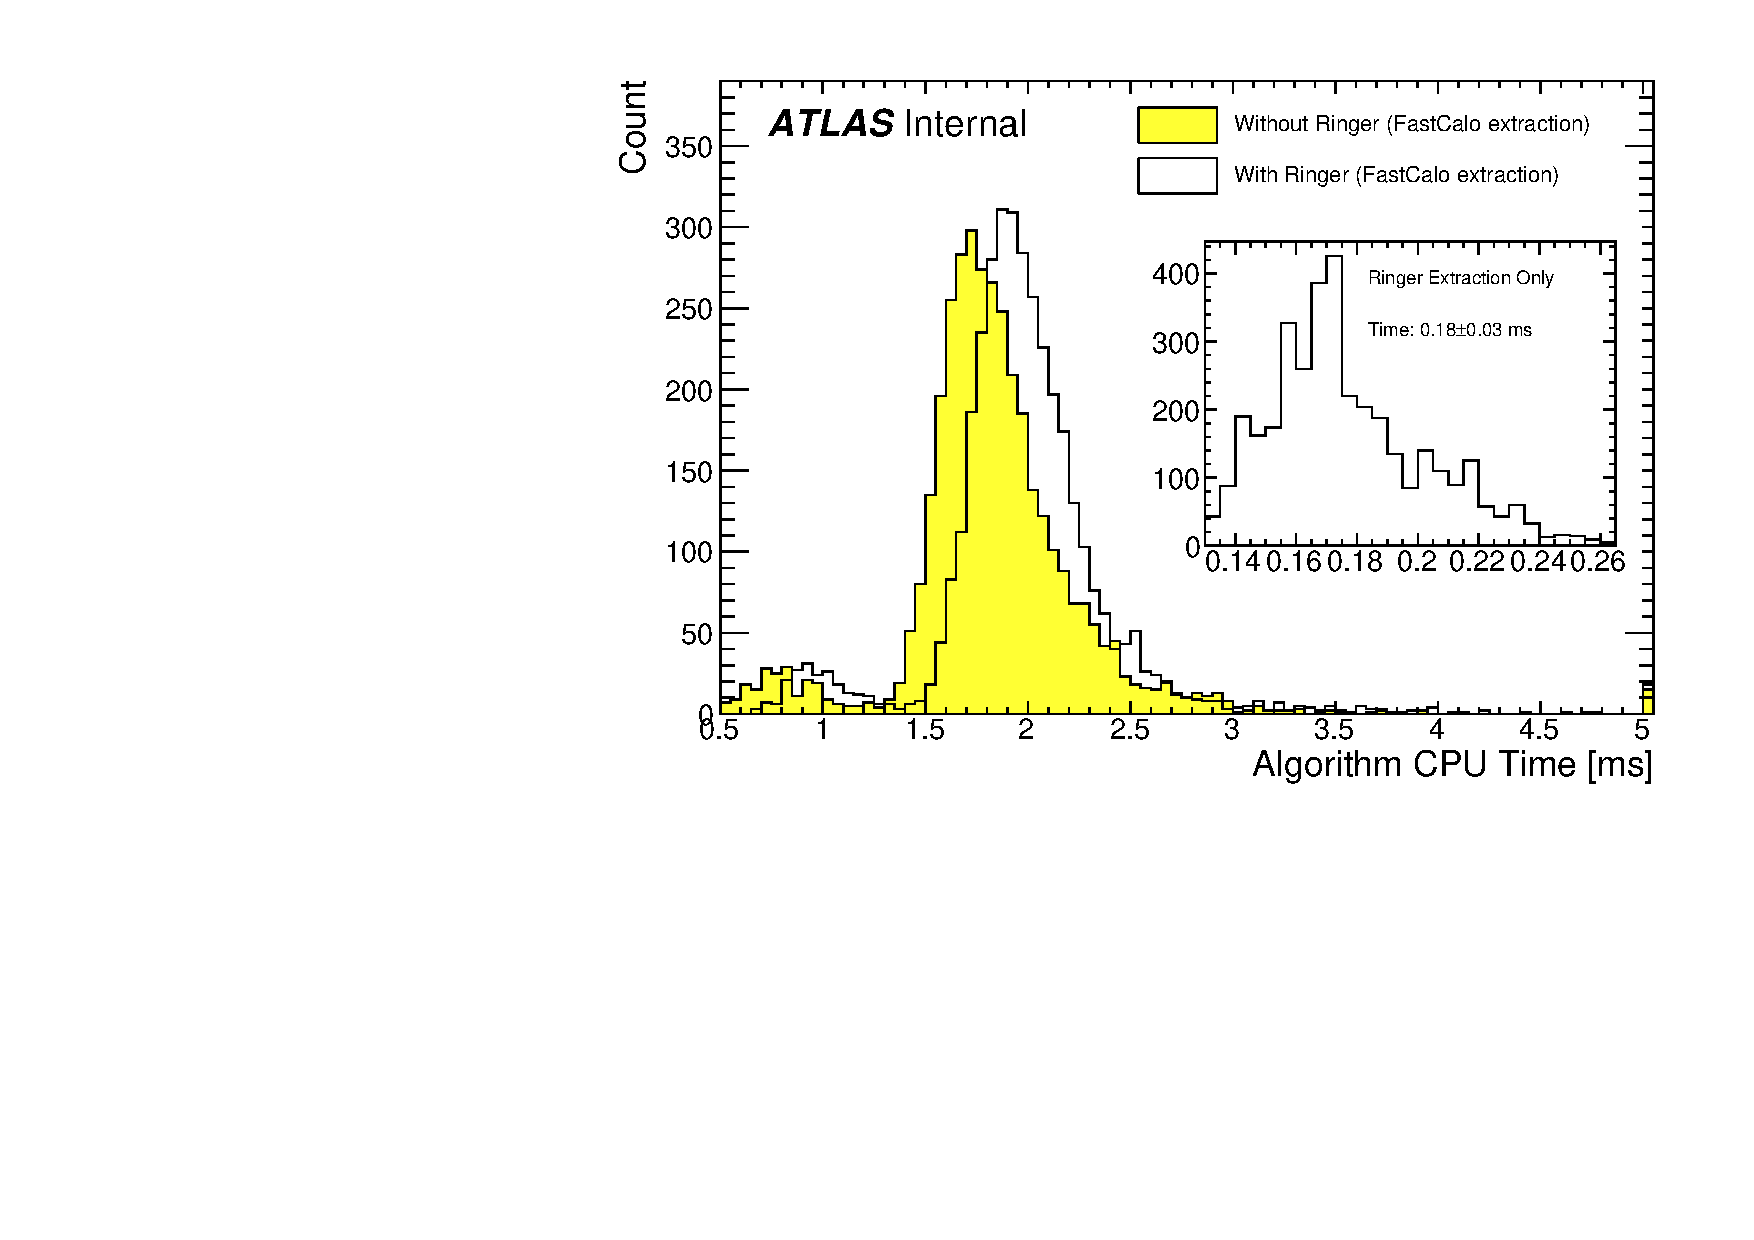
\includegraphics[width=.7\textwidth]{sections/operation/figures/EgammaFex_TotalTime}
% \centering
% \caption{\label{fig:fastcalo_fex_time}
% Total CPU time per bunch-crossing event for the feature extraction algorithms in
% the \fastcalo step of electron triggers with (white) and without (yellow) \rnn{}
% using EB events (see text) in run 327265 ($\avgmu=45$ peak). Detail on right
% shows the CPU time of the ring variable extraction. The CPU time does not
% include the (online) data preparation time.  Measurements were evaluated from
% release AthenaP1-21.1.55 with a single electron trigger (e\_17\_lhvloose\_nod0)
% and with individual executions (independent measurements) in the same dedicated
% TDAQ node.
% }
% \end{figure}

% \begin{figure}[h!tb]
%   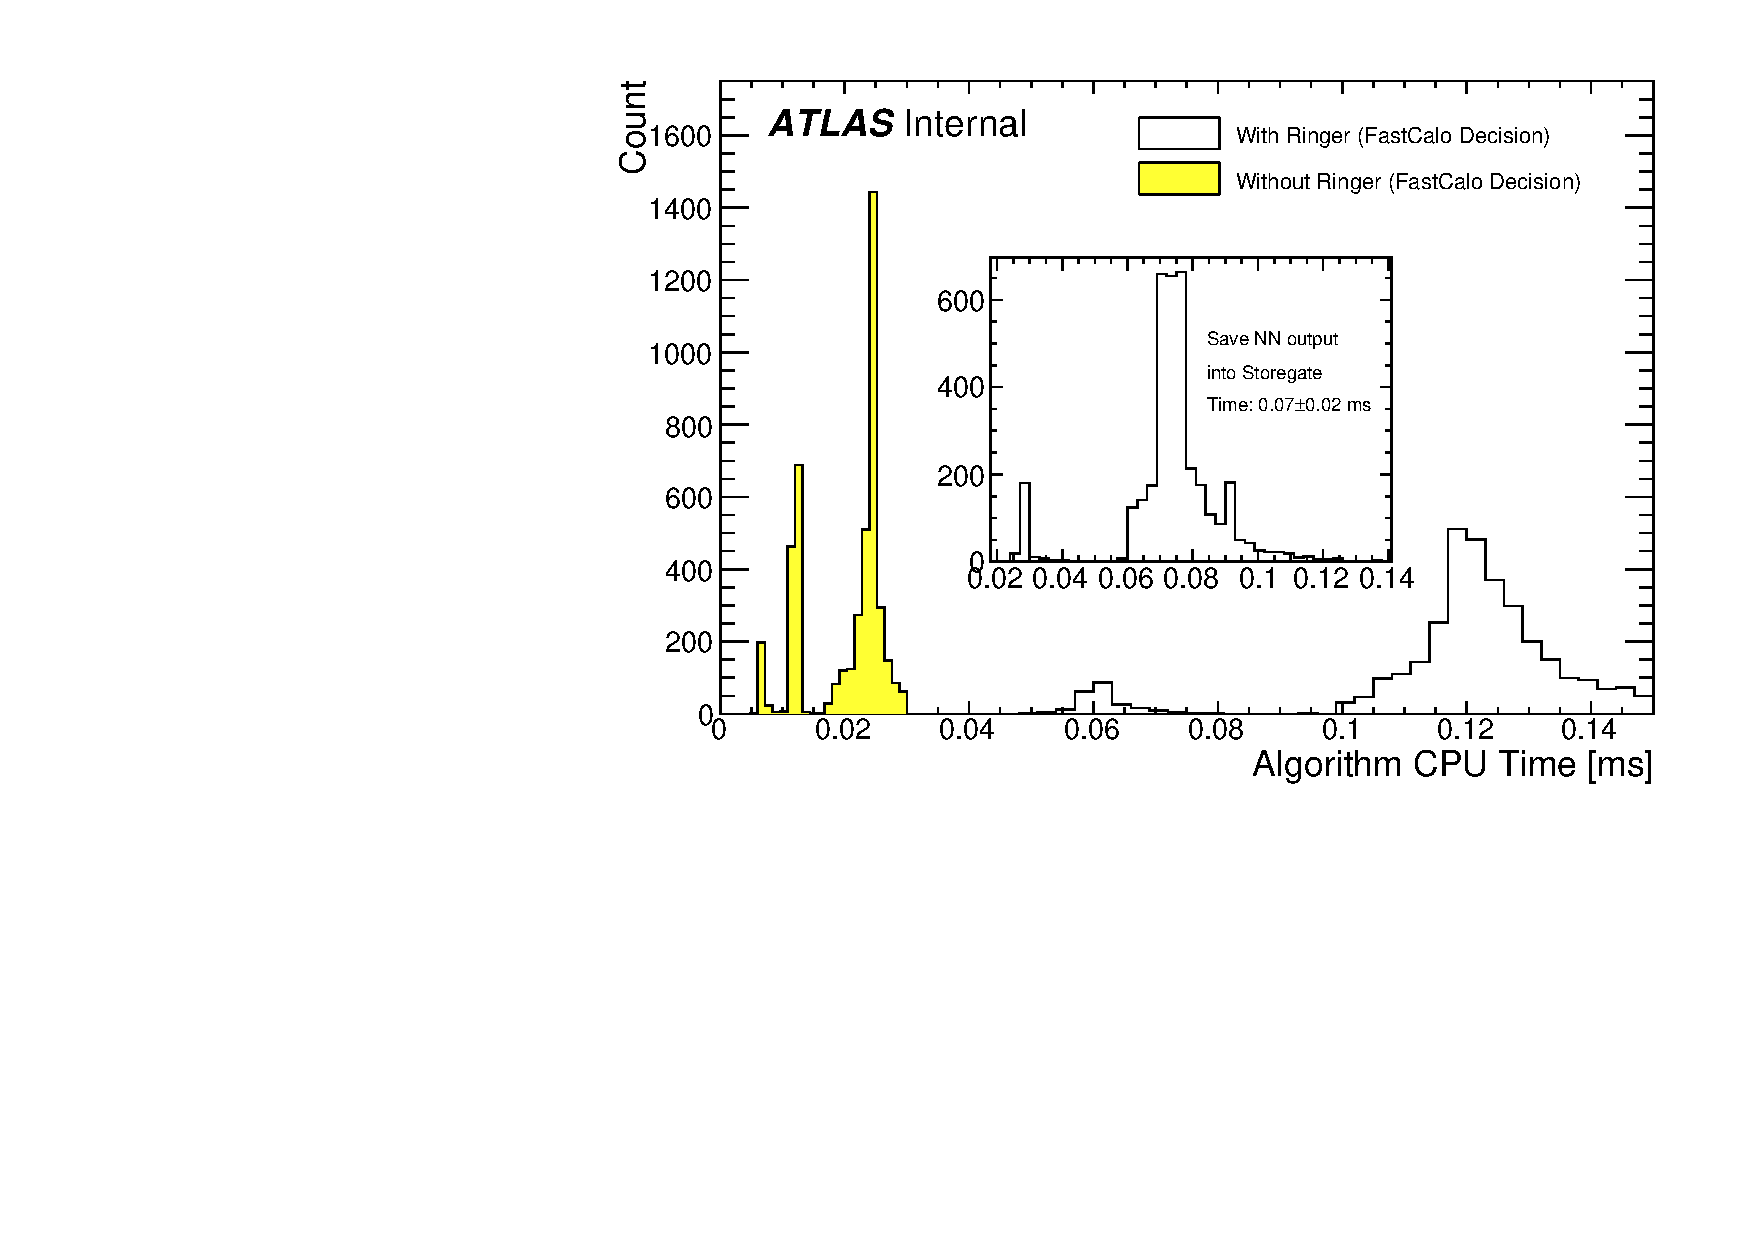
\includegraphics[width=.7\textwidth]{sections/operation/figures/EgammaHypo_TotalTime.pdf}
% \centering
% \caption{\label{fig:fastcalo_hypo_time}
%   Total CPU time per bunch-crossing event for the hypothesis testing algorithms
% in the \fastcalo step of electron triggers with (white) and without (yellow) \rnn{}
% using EB events. More details in description of Figure~\ref{fig:fastcalo_fex_time}. 
% The center histogram represents the CPU time to store the \rnn{} output into the AOD 
% format (persistence).}
% \end{figure}

% A multi-modal structure can be observed in the feature extraction distributions
% of both trigger configurations, which is associated to the algorithm
% for retrieving the EM2 cells and building related shower shape
% variables\footnote{The three peak structure comes from the raw data conversion.
% 	Particularly, these are amongst the most-demanding contributions to
% 	the \fastcalo total CPU time.}. The computation of the ring variables, the only difference between the
% triggers in the \fastcalo feature extraction, requires additional CPU time per
% event of \SI{0.18 \pm 0.03}{\ms/\text{event}}. 
% A less relevant contribution
% comes from hypothesis testing, in which the ring variables are normalized, the
% discriminant is computed, compared to the selection requirement and stored into
% the AOD\footnote{For Run-3 this step has been removed as a way to reduce the CPU time at \fastcalo step.} 
% persistent format. 
% Specifically, \rnn{} hypothesis testing is considerably more demanding
% (up to \SI{0.14}{\ms/\text{event}}), mostly due to the time 
% to store the neural network output \SI{0.07 \pm 0.02}{\ms/\text{event}}, 
% than the cut-based selection
% (\SI{0.02}{\ms/\text{event}}), however small with respect to the feature
% extraction values. 


% Taking into account the referred values, the \rnn{} can require a
% relative increase of up to \SI{50}{\%} in the \fastcalo{} CPU time per event
% with respect to the trigger without \rnn{}\footnote{We expect the result to be
% dependent on the trigger configuration due to presence of pile-up. Reported
% results are for e17\_lhvloose\_nod0.}. Nonetheless, the \rnn{} contributes to
% a more discriminant selection, allowing to obtain less CPU demanding triggers
% by reducing the processing of fake electron in the computationally demanding
% subsequent steps as will be shown in the following sections.

% \FloatBarrier
% \subsubsection{Estimated CPU Impact for the Lowest-Energy Threshold Unprescaled
% Single Electron Trigger}\label{top:cpu_e26}

% We demonstrate the potential of saving CPU requirements by
% avoiding the computation of fake candidates with the \rnn{} algorithms using the
% lowest-energy-threshold unprescaled single electron trigger
% (e26\_lhtight\_nod0\_ivarloose). We executed it with and without the \rnn{}
% algorithm in the same database using a dedicated node for processing.
% In this measurement, we considered about 3,400 events from EB stream of run
% 327265 processed by release AthenaP1,21.1.55. The \rnn{} algorithm provided a
% \SI{60}{\%} reduction (\SI{30.72}{\milli\second} to \SI{10.36}{\milli\second})
% in the CPU demands.


  